\chapter{The LHC and the ATLAS Detector}
\label{sec:det}

\section{The Large Hadron Collider (LHC)}
\label{sec:det-LHC}

High-energy particle colliders have been an essential tool in high-energy physics research for over 50 years,
with a rich history of discovering new particles as each generation of collider pushes the energy frontier;
including the discovery of the $Z$ and $W$ bosons using the Super Proton Synchotron at CERN in 1983~\cite{det-Wdisc_UA1, det-Zdisc_UA1, det-Wdisc_UA2, det-Zdisc_UA2} 
and the discovery of the  top-quark at the Tevatron in 1995~\cite{det-tdisc_CDF, det-tdisc_D0}.

The Large Hadron Collider (LHC) is the highest energy collider ever built,
operated by the \textit{Conseil Europ\'een pour la Recherche Nucl\'eaire (CERN)}.
Lying in a tunnel \SI{100}{\metre} beneath the Swiss/French border near Geneva,
the LHC is a \SI{27}{\km} circumference ring of superconducting magnets and accelerating structures,
which accelerate beams of protons to a maximum energy of \SI{6.5}{\TeV}.
The proton beams are collided in four different locations on the LHC ring
and around each collision point a different detector is constructed to observe these collisions;
one of these detectors is the ATLAS detector.

\subsection{LHC running conditions in 2015 and 2016}

Since May 2015 the LHC has been colliding bunches of protons at a centre-of-mass energy of \SI{13}{\TeV},
the highest energy collisions ever obtained by a particle collider
\footnote{The period of data-taking starting in 2015 and scheduled to continue until the end 2018 is known as Run-2.}.
In 2015 and 2016 the LHC produced $pp$ collisions 
with a bunch spacing of \SI{25}{\nano\second}~\footnote{A small amount of data in 2015 was collected with a bunch spacing of \SI{50}{\nano\second}}.

\textit{Integrated luminosity}, $L$, is the quantity that describes the size of a data-set from a collider experiment.
Integrated luminosity is defined as $L = N_{evt}/\sigma$,
where $\sigma$ is the cross-section of a particular process occurring at that collider experiment
and $N_{evt}$ is the number of events in the data-set that occur through that process.
Instantaneous luminosity, defined as $dL/dt$, % $\frac{dL}{dt}$,
is the rate of data-collection.
An integrated luminosity of \SI{3.9}{\fb^{-1}} and \SI{35.6}{\fb^{-1}} was recorded by ATLAS in 2015 and 2016 respectively~\cite{det-ATLAS_lumi_twiki}.

%Figure \ref{fig:det-lumi_2015_2016} shows the integrated luminosity delivered by the LHC and recorded by ATLAS in 2015 and 2016;

To achieve high instantaneous luminosity at the LHC, bunches of protons are collided resulting in many collisions per bunch-crossing.
%Figure \ref{fig:det-mu_2015_2016} shows the luminosity-weighted distribution of the mean number of interactions per crossing ($<\hspace{-3pt}\mu\hspace{-3pt}>$)
%for 13~TeV proton--proton collision data collected by ATLAS in 2015 and 2016.
The mean number of collisions per bunch-crossing ($<\hspace{-3pt}\mu\hspace{-3pt}>$) depends on the running conditions of the LHC.
For ATLAS, the luminosity weighted average of $<\hspace{-3pt}\mu\hspace{-3pt}>$ is 13.7 in 2015 data and 24.9 in 2016 data~\cite{det-ATLAS_lumi_twiki}.
Collisions in addition to the collision of interest
\footnote{ The position of the collision of interest is known as the primary vertex;
  the experimental definitions of primary vertex (and therefore the collision of interest) is discussed in Section~\ref{sec:obj-tracks_pv}.}
are collectively referred to as \textit{`pile-up'}~\cite{det-pileup}.
Pile-up presents a challenge to physics analyses at the LHC
as the resulting particles from pile-up collisions can affect the measurement of particles from the collision of interest.

%\begin{figure}[!ht]
%  \begin{center}
%    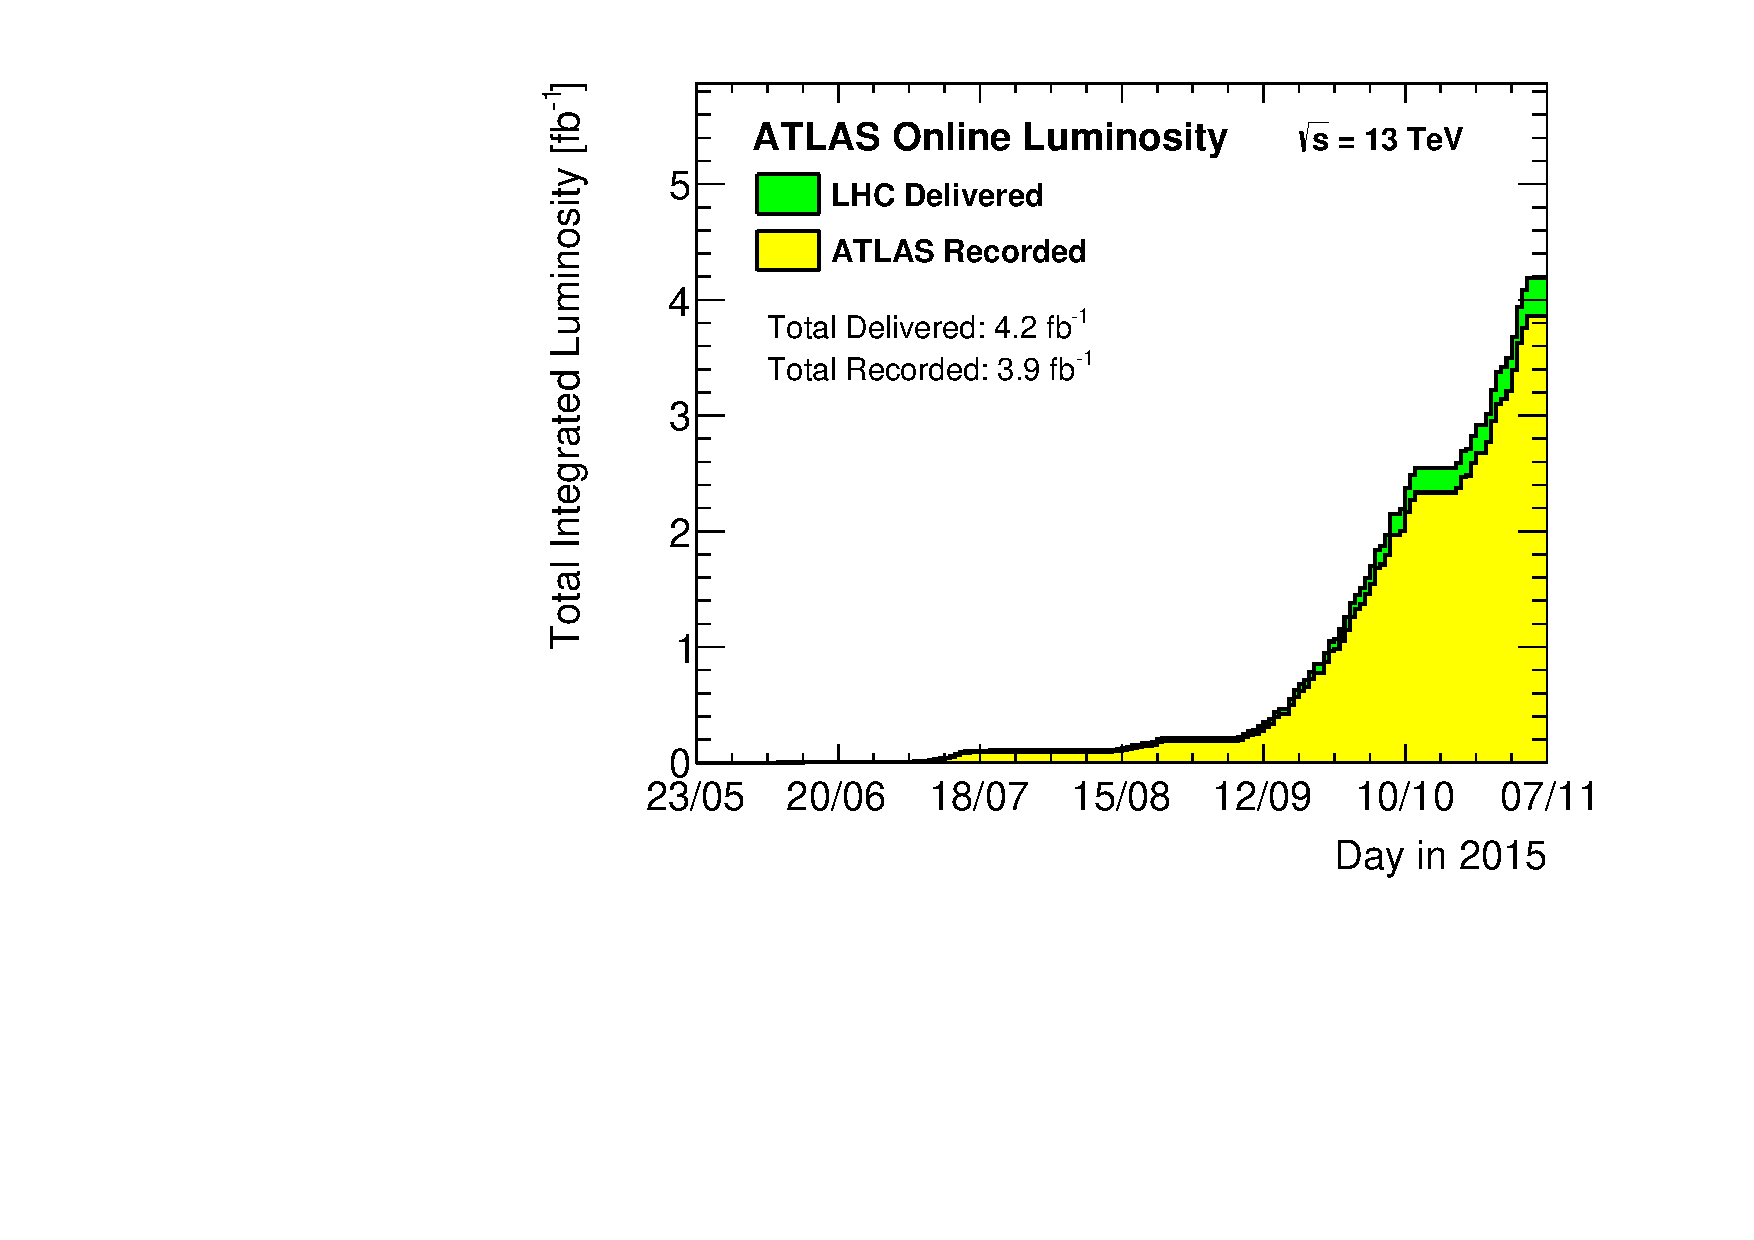
\includegraphics[width=0.4\linewidth, angle=0]{figs/Detector/lumi_2015.pdf}
%    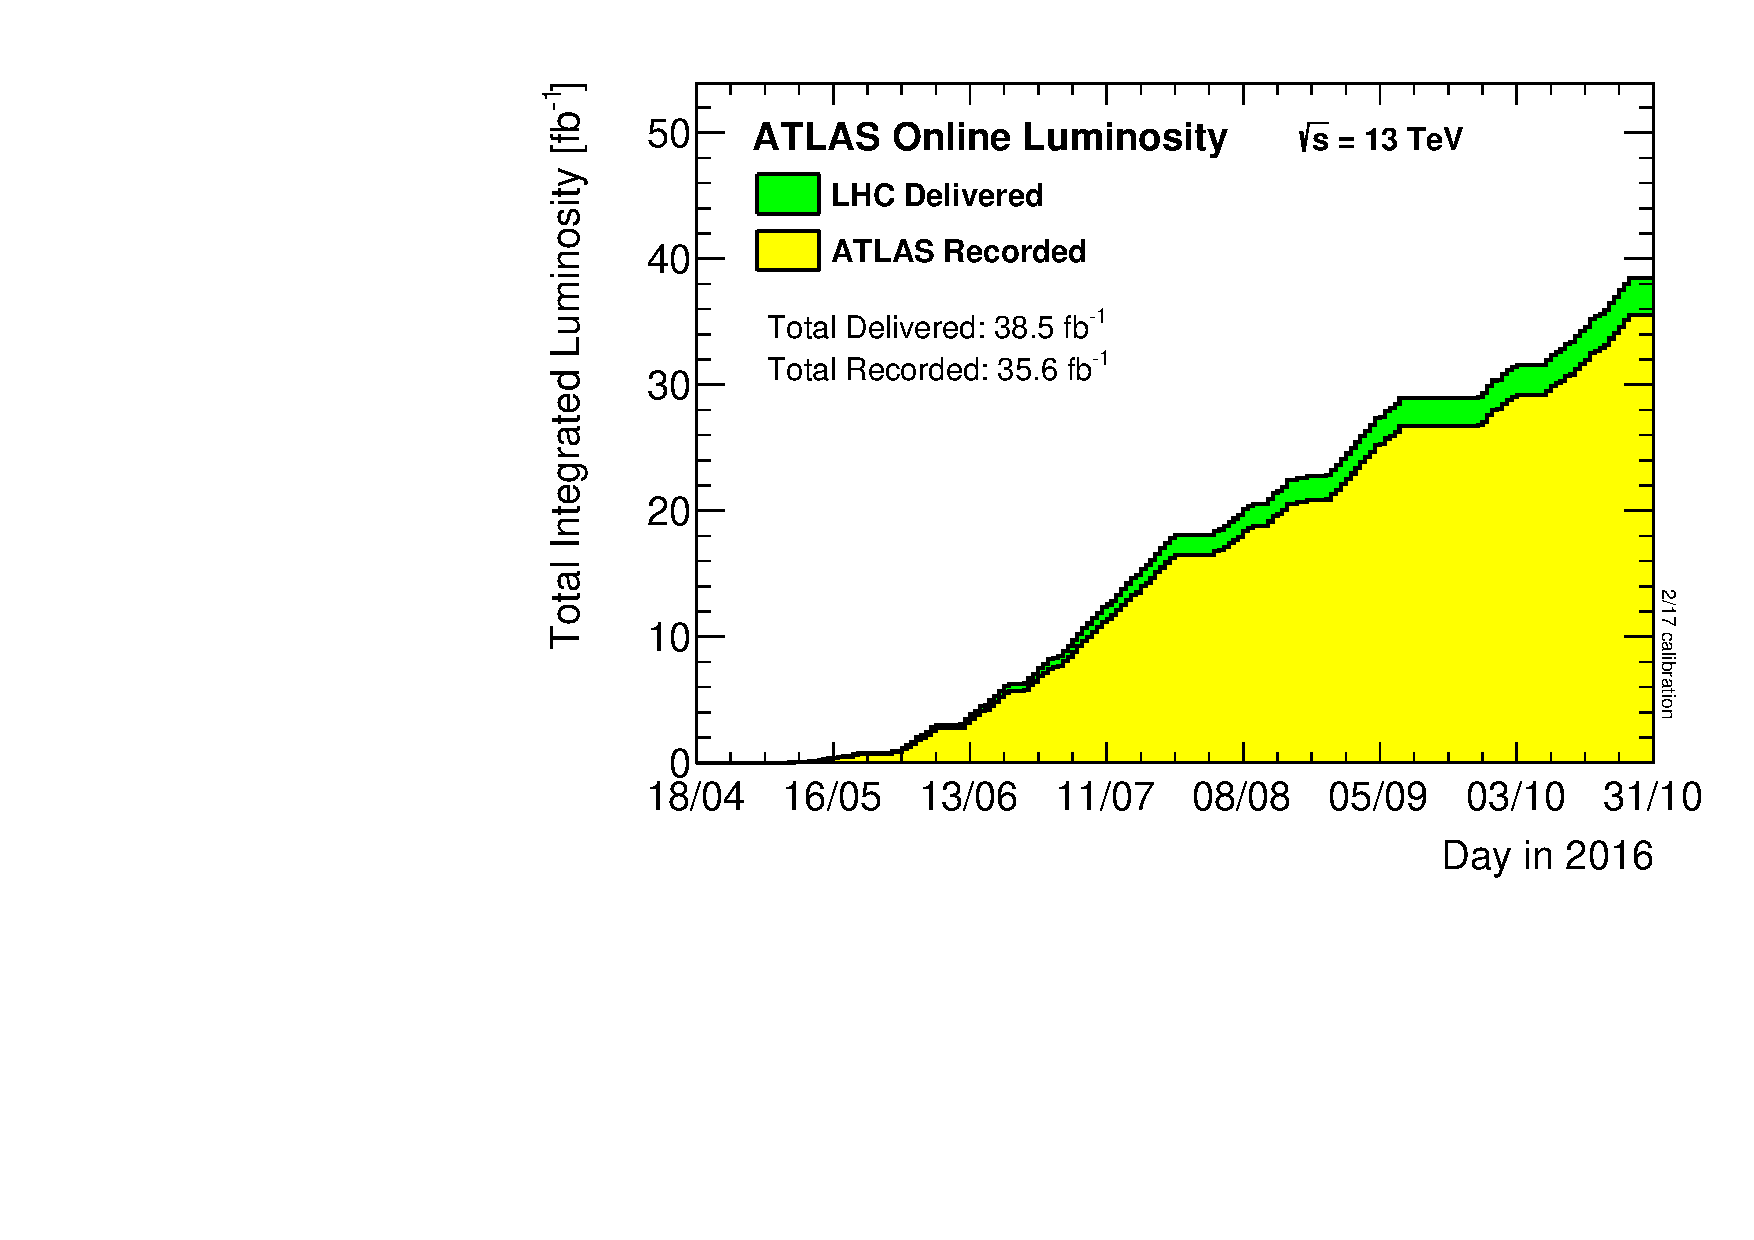
\includegraphics[width=0.4\linewidth, angle=0]{figs/Detector/lumi_2016.pdf}
%  \end{center}
%  \vspace{-1em}
%  \caption[Integrated luminosity delivered to and recorded by ATLAS during 2015 and 2016]
%          {\label{fig:det-lumi_2015_2016}Integrated luminosity versus time delivered to (green) and recorded by ATLAS (yellow) during stable beams for $pp$ collisions
%            at 13 TeV centre-of-mass energy \mbox{in (a) 2015 and (b) 2016~\cite{det-ATLAS_lumi_twiki}.}}
%  \begin{center}
%    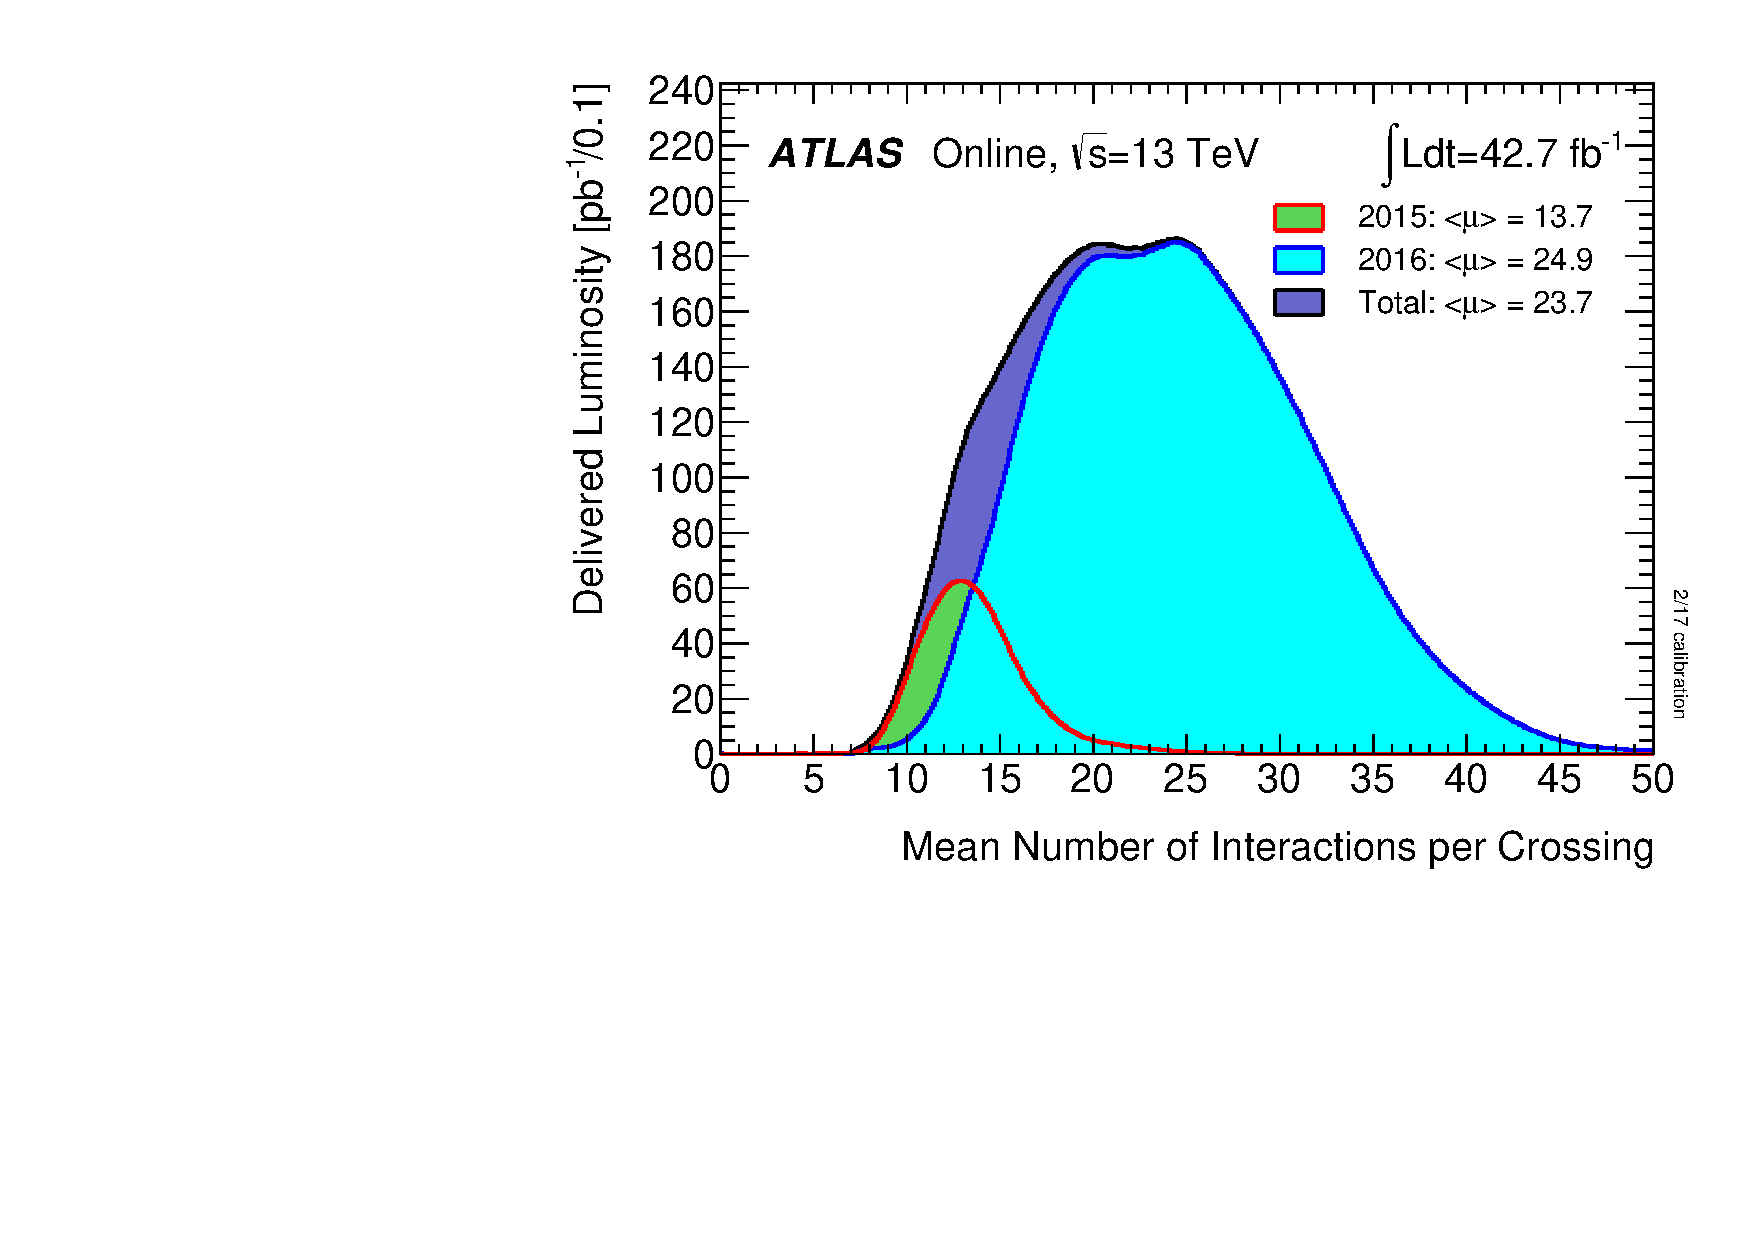
\includegraphics[width=0.4\linewidth, angle=0]{figs/Detector/mu_2015_2016.pdf}
%  \end{center}
%  \vspace{-1em}
%  \caption[The luminosity-weighted distribution of the mean number of interactions per crossing ($<\hspace{-3pt}\mu\hspace{-3pt}>$)
%    for 13~TeV proton--proton collision data collected by ATLAS in 2015 and 2016.]
%          {\label{fig:det-mu_2015_2016} The luminosity-weighted distribution of the mean number of interactions per crossing ($<\hspace{-3pt}\mu\hspace{-3pt}>$)
%            for 13~TeV proton--proton collision data collected by ATLAS in 2015 (green), 2016 (cyan) and 2015-2016 combined (dark blue)~\cite{det-ATLAS_lumi_twiki}.
%          The luminosity-weighted mean number of collisions is shown in the legend.}
%\end{figure}


\section{ATLAS Detector Description}
\label{sec:det-ATLAS}

The ATLAS (\textbf{A} \textbf{T}oroidal \textbf{L}arge Hadron Collider \textbf{A}pparatu\textbf{S}) detector
design, construction and performance has been described in detail in~\cite{det-ATLAS_Exp, det-ATLAS_TDR, det-ATLAS_Perf}.
Therefore this chapter provides a general description of the detector with a focus on the needs of di-$b$-jet searches.
Figure~\ref{fig:det-ATLAS_schem} shows a cut-away schematic of the ATLAS detector.

\begin{figure}[!htb]
  \begin{center}
    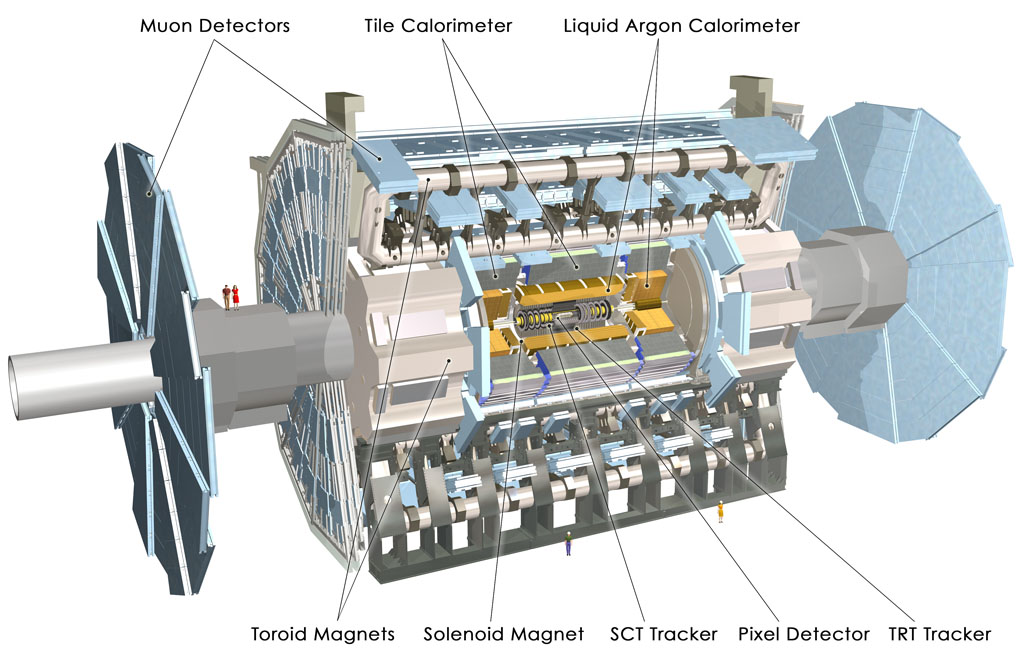
\includegraphics[width=1\linewidth, angle=0]{figs/Detector/ATLAS_schem.jpg}
  \end{center}
  \caption[A cut-away schematic of the ATLAS detector.]{ A cut-away schematic of the ATLAS detector~\cite{det-ATLAS_Exp}.}
  \label{fig:det-ATLAS_schem}
\end{figure}

\clearpage
The ATLAS detector is a large closed cylindrical detector,
consisting of a system of magnets and three sub-detectors; the Inner Detector, the Calorimeter system and the Muon Spectrometer.
The magnets and sub-detectors sit in concentric rings around the interaction point, where the proton bunches collide.
Combining the measurements from each of the sub-detectors allows the 
ATLAS detector to identify and measure the key properties~\footnote{\ For example four-momentum.}
of particles that pass through its volume.
Each component of the ATLAS detector is described in further detail below.

%and Figure~\ref{fig:det-ATLAS_slice} shows a slice of the detector in the plane perpendicular to the beam-pipe,
%overlaid are simplified illustrations how the detector responds to a range of particles~\cite{det-thesis_gutchow}.


%\begin{figure}[!ht]
%  \begin{center}
%    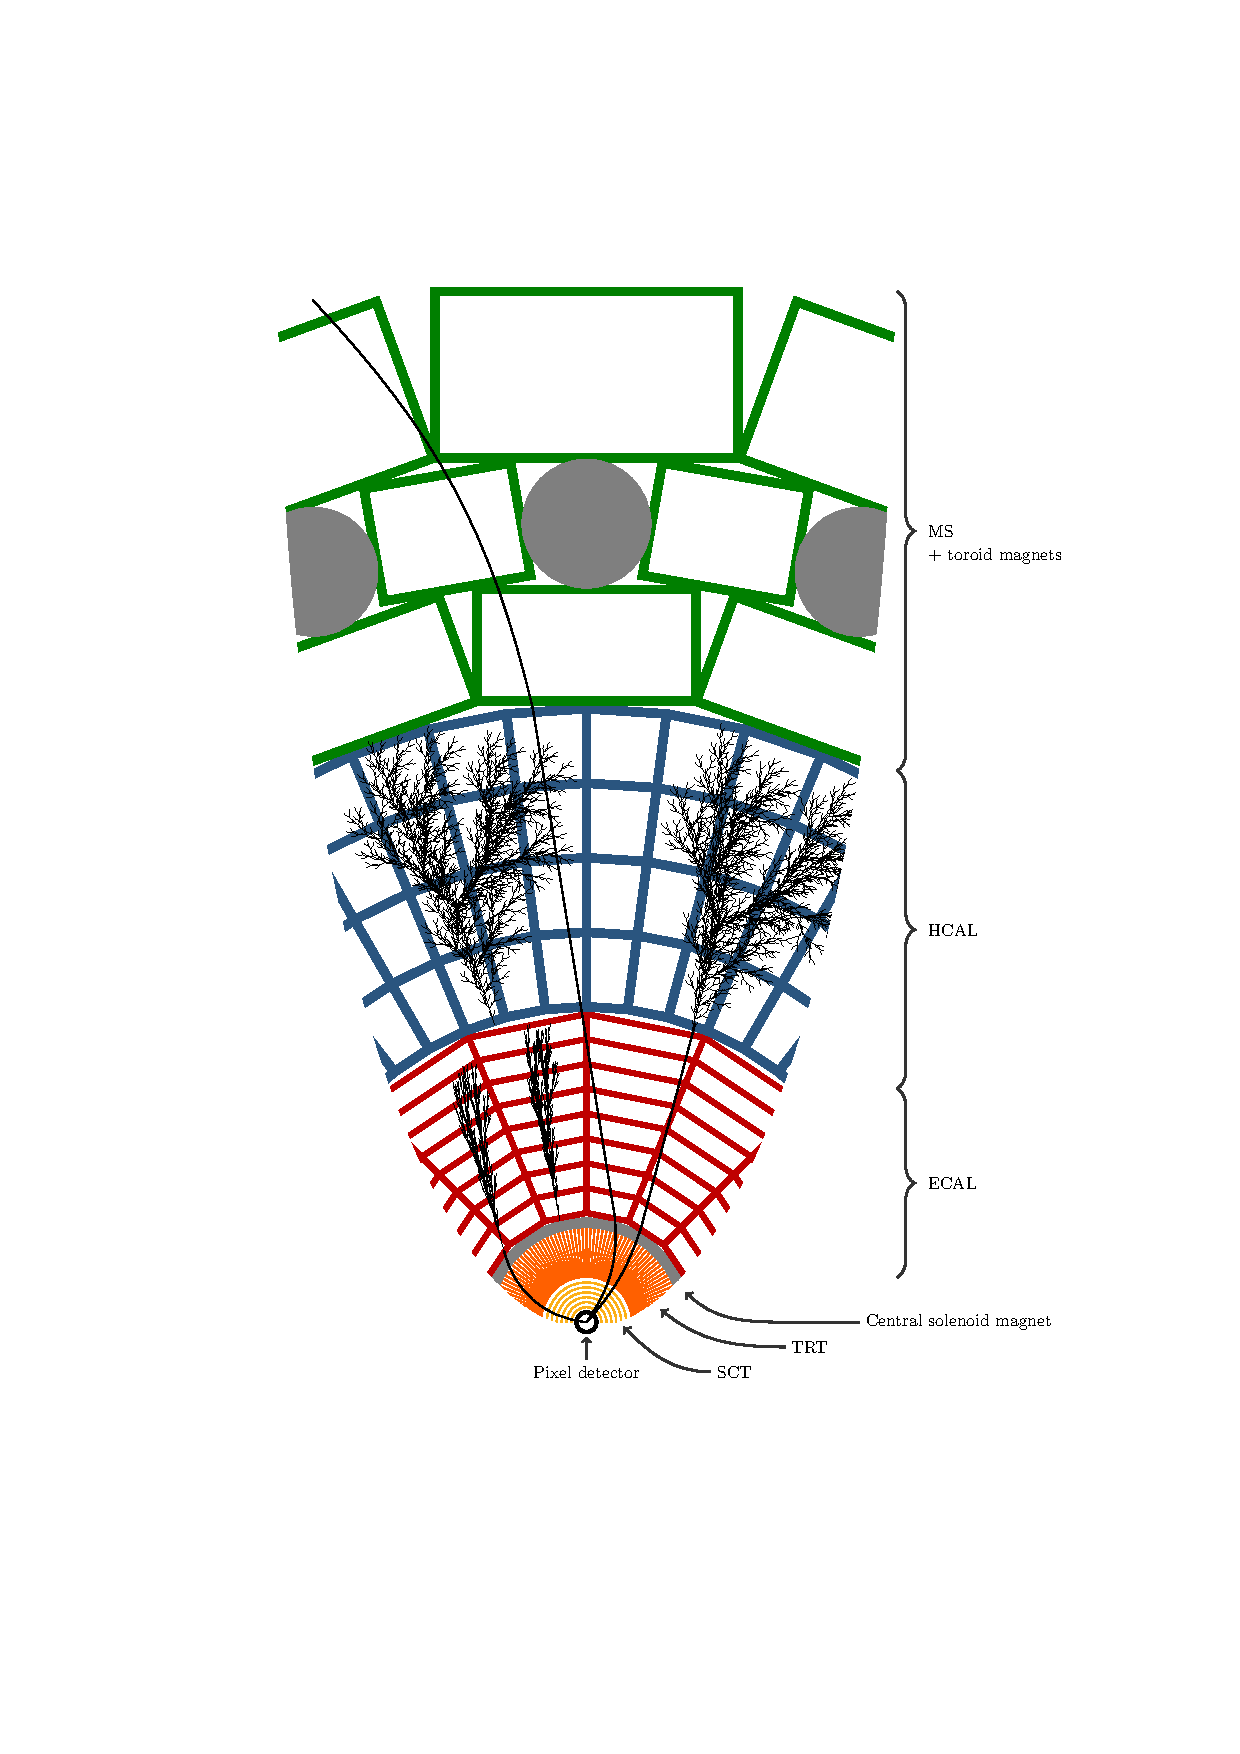
\includegraphics[width=0.7\linewidth, angle=0]{figs/Detector/ATLAS_slice.pdf}
%  \end{center}
%  %When citing in a caption, use this set-up
%  \caption[A visualisation of the ATLAS detector and the various sub-detectors with simplified illustrations of how various types of particles interact with the ATLAS detector overlaid.]
%          {A visualisation of the ATLAS detector and the various sub-detectors.
%    The view is taken as a slice in a plane perpendicular to the beam-pipe,
%    showing the radial range from the beam-pipe to the edge of the detector.
%    Overlaid are simplified illustrations of how various types of particles interact with the ATLAS detector;
%    specifically from left to right the particles are an electron, a chargeless hadron (e.g. a neutron), a photon, a muon and a charged hadron (e.g. proton).
%    The sub-detector components are not to scale~\cite{det-thesis_gutchow}.}
%  \label{fig:det-ATLAS_slice}
%\end{figure}

\subsection{ATLAS Co-ordinate System}
\label{sec:det-coordinate}

%Firstly, to describe the detail of the ATLAS detector there must be a description of the co-ordinate system that is used.
ATLAS uses a right-handed coordinate system, in which the origin lies at the interaction point.
The $x$-axis points towards the centre of the LHC ring parallel to the surface of the earth,
the $y$-axis points vertically upwards towards the surface of the earth
and the $z$-axis runs along the beam-pipe, pointing anti-clockwise along the LHC beam-pipe.
The azimuthal angle, $\phi$, is defined right-handedly around the $z$-axis starting at the $x$-axis.
%Figure~\ref{fig:det_coordinate} illustrates this co-ordinate system.

The polar angle, $\theta$, is defined as the angle measured from the $z$-axis,
such that along the $z$-axis corresponds to $\theta = 0$
and anti-aligned with the $z$-axis corresponds to $\theta = \pi$.
From that pseudorapidity, $\eta$, is defined as:
\begin{equation}
 \eta = -\ln\left[\tan\left( \frac{\theta}{2} \right) \right]
\end{equation}
Thus, $\eta = 0$ corresponds to a particle travelling perpendicular to the beam-pipe,
where a positive value of $\eta$ corresponds to a particle travelling with a tilt towards the positive $z$-axis.
The quantity is called pseudorapidity as in the massless limit (when $|\vec{p}| \to E$)
it can be shown that $\eta$ converges to rapidity, $y$, where rapidity is defined as,
\begin{equation}
  y = \frac{1}{2} \ln \left( \frac{E+p_{z}}{E-p_{z}} \right)
\end{equation}
A key property of rapidity is that differences in rapidity, $\Delta y$, are invariant against Lorentz boosts along the $z$-axis.
This is important in $pp$ colliders as each collision has  a different Lorentz boost along the $z$-axis,
due to the effects of the Parton Distribution Functions described in Section~\ref{sec:theo-qcd_pdf}.
This implies that, in the massless limit, $\Delta \eta$ is also invariant against Lorentz boosts along the $z$-axis.
Therefore $\eta$ is used to define the angular direction with respect to the z-axis in the ATLAS co-ordinate system.

The final important quantity of the ATLAS co-ordinate system is $\Delta R$, which is defined as $\Delta R = \sqrt{\Delta\eta^{2} + \Delta\phi^{2}}$.  
\Delta R represents the angular separation between two vectors.


%Now that we have discussed the ATLAS co-ordinate system, we can provide a description of the components of the ATLAS detector.

\subsection{Inner Detector}
\label{sec:det-ID}

The innermost ATLAS sub-detector is the Inner Detector (ID) which
measures the trajectory of charged particles.
The ID is constructed from many concentric layers of detectors.
As a charged particle passes through the ID, each of the layers provide a position measurement known as a hit.
A particle passing through the whole ID at $\eta=0$ will typically cause 44 hits. % 4+4+36
The trajectory of the particle is determined using the hits from each of the layers,
the measured trajectory is known as a track. Track reconstruction will be discussed further in Section~\ref{sec:obj-tracks}.
The ID is immersed in a 2~T magnetic field which bends the trajectories of charged particles;
the sign of the charge and the momentum of the particle is inferred from the sign and magnitude of the track's curvature.

The ID consists of four components; the Insertable B-Layer (IBL), the pixel detector, %~\footnote{\ Often the IBL is considered as part of the pixel detector.},
the Semi-Conductor Tracker (SCT) and the Transition Radiation Tracker (TRT).
The ID measures the position of particles in the angular range $|\eta|\nobreak<\nobreak2.5$;
to achieve this the ID components are organised into the barrel, which are cylinders around the beam-pipe in the central region %\footnote{ Central here means at a low value of $|z|$}
of the detector, and the end-caps, which are disks that lie perpendicular to beam-pipe on either end of the barrel.
Table~\ref{tab:det-ID} summarises the key properties of the components of the ID in both the barrel and the end cap.
Figure~\ref{fig:det-ID_slice} shows the components of the ID in the barrel and the radial positions of each of the layers.
Figure~\ref{fig:det-ID_schem} shows the layout of the barrel and end-cap components of the ID (except the IBL) in one half of the detector.

\begin{figure}[!b]
  \begin{center}
    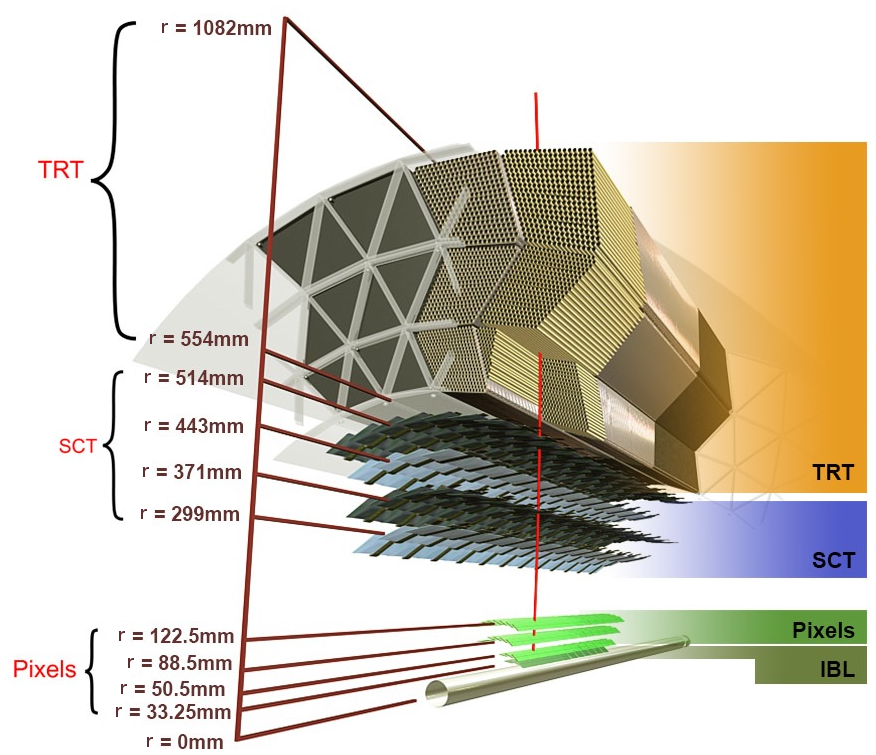
\includegraphics[width=0.7\linewidth, angle=0]{figs/Detector/ID_slice.png}
  \end{center}
  \caption[A schematic showing a slice of the barrel components of the ATLAS Inner Detector including the Insertable $B$-Layer.]
          {A schematic showing a slice of the barrel components of the ATLAS Inner Detector (ID) including the Insertable $B$-Layer (IBL).
            Each component is labelled and the radial distances from the beam-pipe ($r$) is shown~\cite{obj-tracks_TIDE}.}
  \label{fig:det-ID_slice}

  \begin{center}
    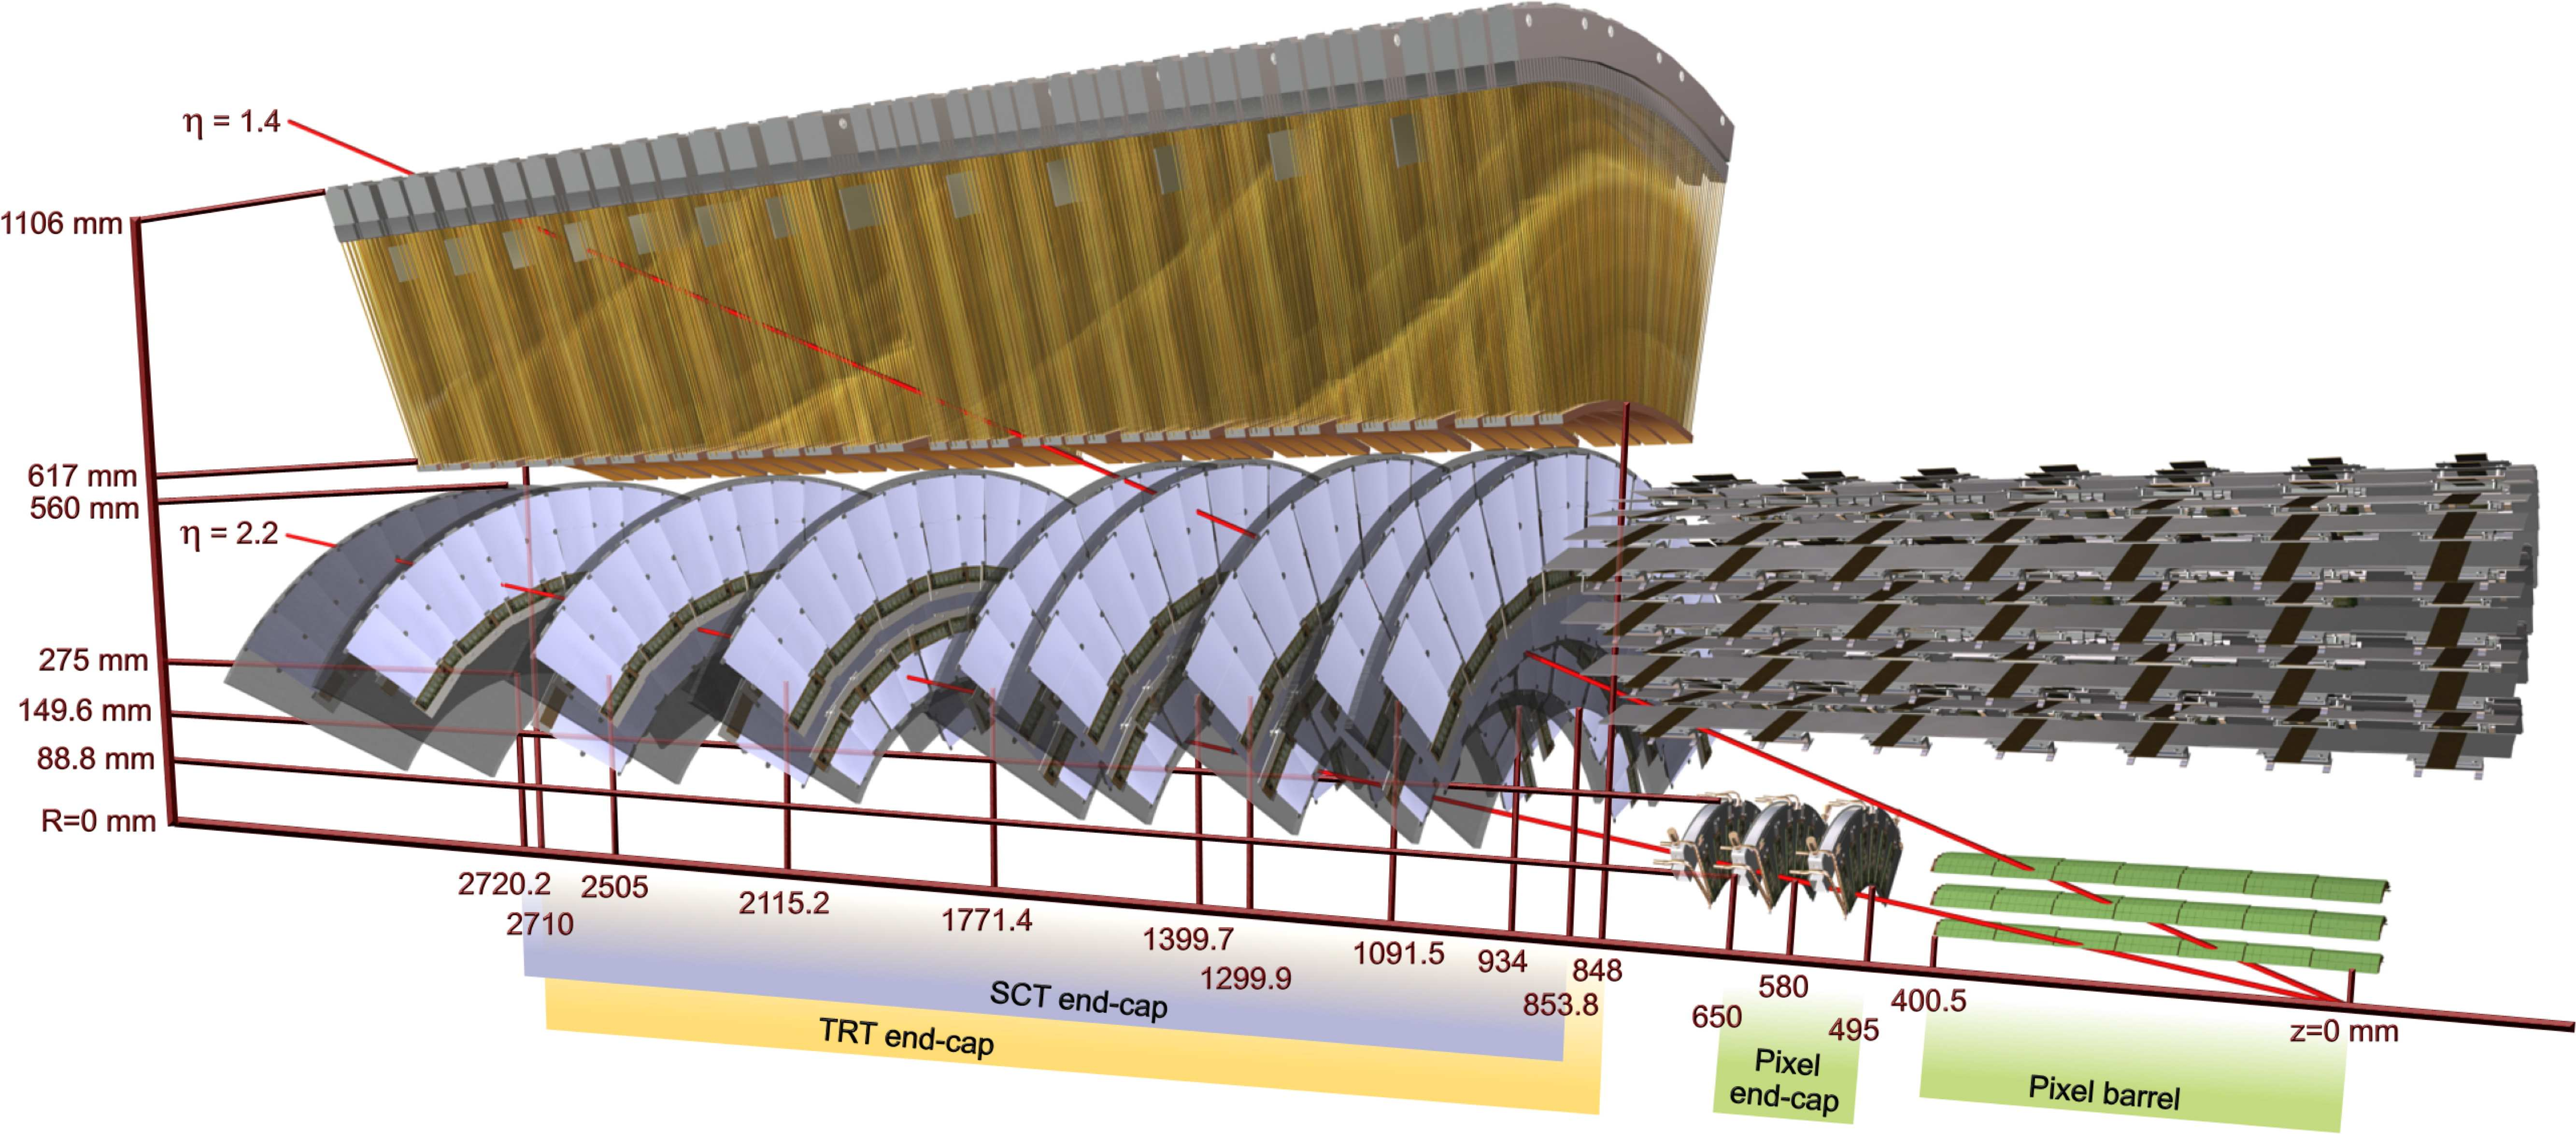
\includegraphics[width=0.9\linewidth, angle=0]{figs/Detector/ID_schem.pdf}
  \end{center}
  \caption[A schematic showing the barrel and end-cap components of the ATLAS Inner Detector.]
          {A schematic showing the barrel and end-cap components of the ATLAS Inner Detector (ID), the Insertable $B$-Layer is not shown.
            Each component  is labelled and the axial distance from the beam-pipe ($z$) is shown.
            The red lines indicate the trajectory of a particle at $\eta$ = 1.4 and 2.2 with $p_T$ = 10 GeV.~\cite{det-ATLAS_Exp}.}
  \label{fig:det-ID_schem}
\end{figure}


%\begin{figure}[!ht]
%  \begin{center}
%    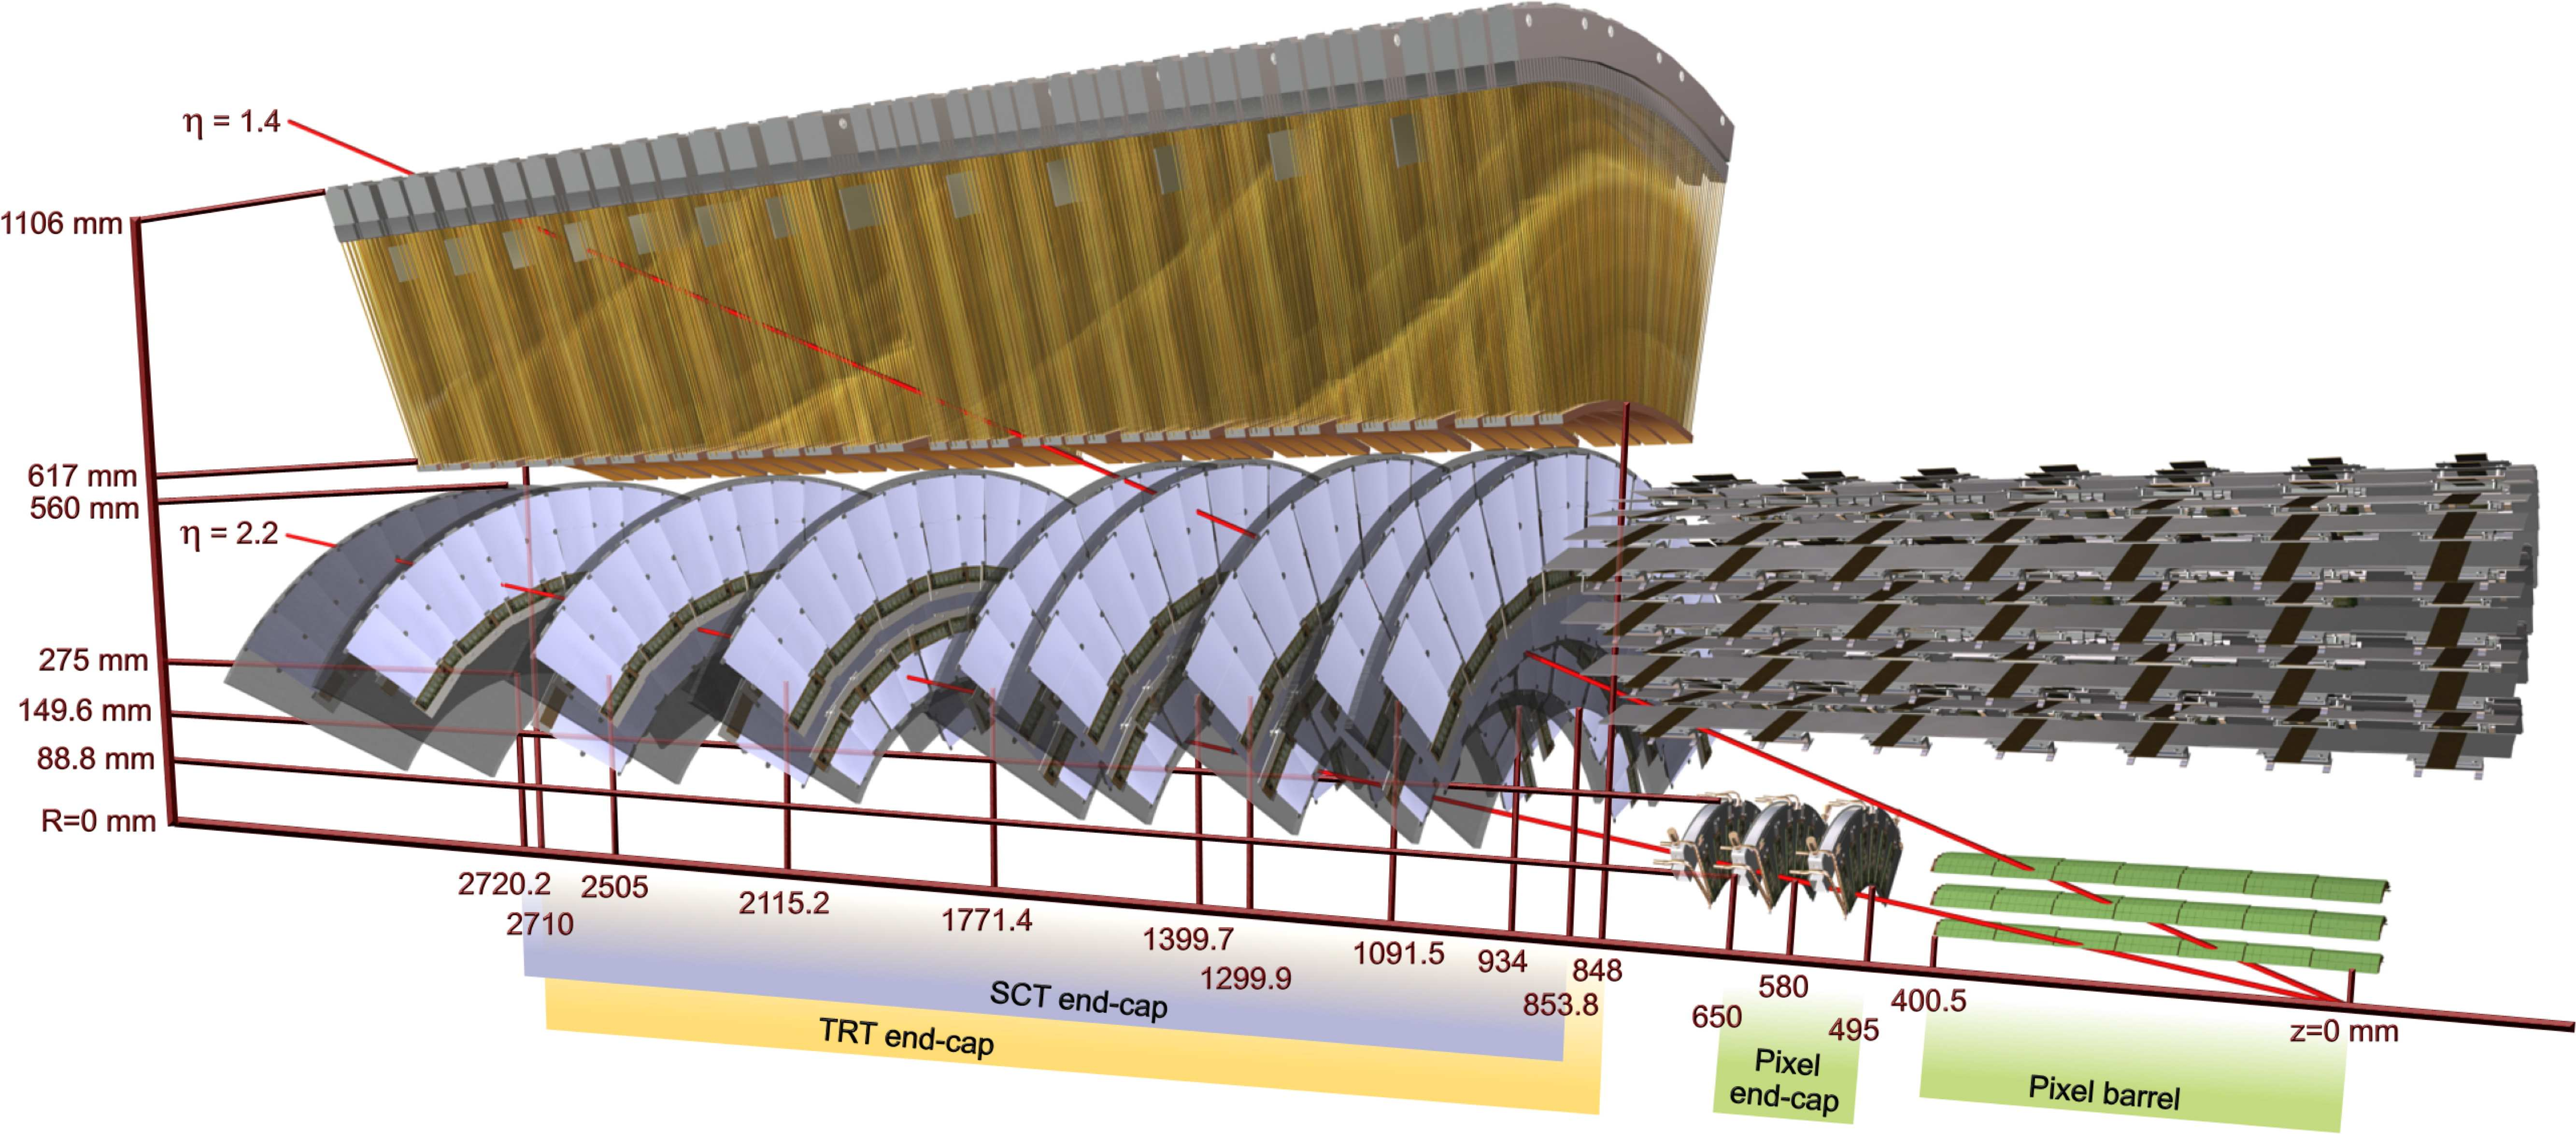
\includegraphics[width=0.8\linewidth, angle=0]{figs/Detector/ID_schem.pdf}
%  \end{center}
%  \caption[A cut-away schematic of the ATLAS Inner Detector (ID).]
%          {A cut-away schematic of the ATLAS Inner Detector (ID)~\cite{det-ATLAS_Exp}.}
%  \label{fig:det-ID_schem}
%\end{figure}

{\renewcommand{\arraystretch}{1.1}
  \begin{table}[!htb]
    \vspace{-0.2em}
\centering
\begin{tabular}{|cc||c|c|rr|c|}
  \hline
  \multicolumn{2}{|c||}{\textbf{Component}} & \multirow{2}{*}{\textbf{$\eta$ Coverage}} & \textbf{Element} &  \multicolumn{2}{c|}{\textbf{Intrinsic}} & \textbf{\# Layers} \\
  \multicolumn{2}{|c||}{\textbf{of ID}}     &       & \textbf{Size (\SI{}{\micro\metre})}  & \multicolumn{2}{c|}{\textbf{Resolution (\SI{}{\micro\metre})}} &  \textbf{or Disks}          \\
  \hline
  \multirow{2}{*}{\textbf{IBL}} & & \multirow{2}{*}{$|\eta| \lt$  2.5}   & \multirow{2}{*}{50 x 250} & \multirow{2}{*}{8 ($R$-$\phi$)}& \multirow{2}{*}{40 ($z$)}  & \multirow{2}{*}{1} \\ %& 33.25 \\
   &&&&&&\\\hline                                                                                                                                                  
  \multirow{2}{*}{\textbf{Pixel}} & Barrel    &  $|\eta| \lt$  1.7            & \multirow{2}{*}{50 x 400} & 10 ($R$-$\phi$)        & 115 ($z$)          & 3                \\ %& 50.5 -- 122.5    \\
                         & End-cap   &         1.7  $\lt |\eta| \lt$  2.5    &                    & 10 ($R$-$\phi$)        & 115 ($R$)          & 3 (both ends)    \\ %& 88.8 -- 149.6    \\
  \hline                                                                                                                                                
  \multirow{2}{*}{\textbf{SCT}}   & Barrel    & $|\eta| \lt$  1.4             &\multirow{2}{*}{80}       &  17 ($R$-$\phi$)        & 580 ($z$)          & 4                \\ %& 299 -- 514       \\
                         & End-cap   &        1.4  $\lt |\eta| \lt$  2.5    &                   &  17 ($R$-$\phi$)        & 580 ($R$)          & 9 (both ends)    \\ %& 275 -- 560       \\
  \hline                                                                                                                                                
  \multirow{2}{*}{\textbf{TRT}}   & Barrel    & $|\eta| \lt$  0.7             & \multirow{2}{*}{4000}     & \multicolumn{2}{c|}{\multirow{2}{*}{130 ($R$-$\phi$)}}     & $\sim$ 36 hits    \\ %& 563 -- 1066      \\
                         & End-cap   &         0.7  $\lt |\eta| \lt$  2.0    &                  &                         &                  & per track        \\ %& 644 -- 1004     \\
  \hline
\end{tabular}
\caption[Summary of the main characteristics of the components of the ATLAS Inner Detector.]
        {\label{tab:det-ID}Summary of the main characteristics of the components of the ATLAS Inner Detector~(ID).
          For the SCT and TRT the element sizes refer to the spacing of the readout strips and the diameter of the straw tubes respectively~\cite{det-ATLAS_Exp,det-ID_table}.}
         \vspace{-1em}
\end{table}
}

The components of the ID closest to the beam-pipe are the IBL and the pixel detector,
which are both made out silicon based pixel modules.
As shown in Table~\ref{tab:det-ID}, the high-granularity of the IBL and pixel detector allow for high precision position measurements
close to the beam-pipe, the importance of this will be outlined below.
The pixel detector consists of 3 barrel layers and 3 end-cap disks at either end of the ID.
The IBL was added to the ID in 2014 to provide an extra position measurement close to the beam-pipe
and to improve tracking efficiency,
which had been degraded by damage to the other layers of the pixel detector in data-taking before 2014.
The IBL is a single layer of pixel modules in the barrel only, which provides an angular coverage of $|\eta|\nobreak<$ 2.5.

Moving radially outwards, the next component of the ID is the Semi-Conductor Tracker~(SCT).
The SCT modules are made from two parallel layers of semi-conducting strips.
The strips are $\sim$\SI{120}{\mm} in length \footnote{ This number varies for the various parts of the SCT}
and have a strip pitch (spacial separation between strips) of \SI{80}{\micro\metre}.
The parallel strip layers within each module have a 40 mrad angular offset along their common normal
such that each module can produce a 3D position measurement.

The outermost component of the ID is the Transition Radiation Tracker (TRT)
constructed of many \SI{4}{\mm} radius cylindrical tubes filled with a xenon based gas mixture
\footnote{ 70\% Xe, 27\% $\text{CO}_2$ and 3\% $\text{O}_2$~\cite{det-ID_xe}.}
%Xenon is used for its high efficiency to absorb TR photons of typical energy 6–15 keV.
with an anode wire through the central axis.
A charged particle passing through the gas causes ionisation allowing for a measurement of its position using drift-time.
In addition, the space between the straws is filled with polymer fibres (barrel) and foils (end-caps) to create transition radiation,
which is emitted by relativistic charged particles as they pass a boundary between materials with different refractive indices.
The intensity of the transition radiation is inversely proportional to the mass of the charged particle,
which are used to discriminate between electrons and pions~\cite{det-ID_TR}.
%% Pion vs electron is example

The trajectory, momentum and transition radiation measurements provided by the Inner Detector are essential for particle identification at ATLAS.
In particular, the high precision position measurements close to the beam-pipe from the IBL and pixel detector
are used to identify tracks originating from hadrons containing $b$-quarks, which are then used to identify $b$-jets.
$b$-jet identification is important for di-$b$-jet searches and is described in Section~\ref{sec:obj-bjets}.

\subsection{ATLAS Calorimeter System}
\label{sec:det-calo}

The ATLAS calorimeter system is located on the outside of the solenoid magnet surrounding the ID and
is designed to provide an energy measurement of the traversing particles.
The ATLAS calorimeter is particularly important for di-$b$-jet searches as it measures the
energy of hadronic jets which are used to calculate the invariant mass of jet pairs. %dijet invariant mass,

The ATLAS calorimeter consists of two different systems built in concentric rings;
the innermost is the \textit{`Electromagnetic Calorimeter system'} (ECAL) used to measure electromagnetic objects such as photons and electrons.
Outside of that is the \textit{`Hadronic Calorimeter system'} (HCAL) that provides an energy measurement of hadronic jets.
The HCAL consists of the Tile and Hadronic Endcap calorimeters.
Both the ECAL and HCAL have barrel and end-cap components to make energy measurements at a large range of $\eta$ values.
Figure \ref{fig:det-calo_schem} shows a cut-away of the ATLAS calorimeter.

\begin{figure}[!ht]
  \begin{center}
    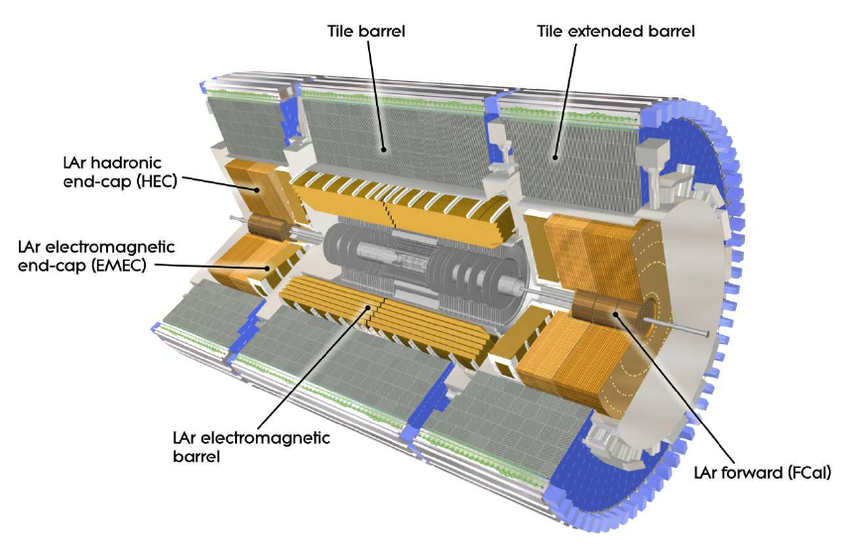
\includegraphics[width=0.8\linewidth, angle=0]{figs/Detector/Calo_schem.png}
  \end{center}
  \caption[A cut-away schematic of the ATLAS calorimeter system.]
          {A cut-away schematic of the ATLAS calorimeter system~\cite{det-ATLAS_Exp}.}
  \label{fig:det-calo_schem}
\end{figure}

A more detailed description of the calorimeter components will follow;
however, the principle behind each component of the calorimeter is common so is described first.
The calorimeters at ATLAS are sampling calorimeters, which means that they consist of alternating layers of absorber and active material.
The role of the \textit{`absorber layer'} is to force the particle, whose energy we want to measure, to emit secondary particles.
These secondary particles will again emit further particles and so on such that a particle cascade is formed,
the many resulting particles from the cascade are known as the cascade particles.
The role of the \textit{`active material layer'} is to measure the energy of the cascade particles %,
by counting electrons released by ionisation or photons emitted by excited atoms.
%the active layers in the ECAL and HCAL operate using different techniques so will be described below.
The ATLAS calorimeter is designed such that the full particle shower of the initial particle occurs within
its volume meaning the total energy of the initial particle is observed.

\subsubsection{Electromagnetic Calorimeter (ECAL)}

For the electromagnetic interaction, at energies above the critical energy (\SI{7}{\MeV} for lead~\cite{obj-bjets_PDG})
the particle cascade process is dominated by two processes;
bremsstrahlung, ($e^{\pm} \to e^{\pm} + \gamma$) and pair production ($\gamma \to e^{+} + e^{-}$).
Below the critical energy the particle cascade process is dominated by ionisation.
As the energy loss per ionisation interaction is approximately the ionisation energy of the active material,
the number of electrons released through ionisation is proportional the energy of the initial particle.

The electromagnetic calorimeter at ATLAS is known as the \textit{`Liquid Argon (LAr) calorimeter'}.
The absorber material used in the LAr calorimeter is lead, due to its large density of charged particles (high Z)
which increases the rate of the cascade processes and reduces the shower depth.
The active material is liquid argon (LAr);
the electrons released through ionisation in the LAr are captured by an electric field and counted
such that the energy of the initial particle can be calculated.

As discussed above the LAr calorimeter is split up into two sections;
the barrel section covers a region of $|\eta|\nobreak<\nobreak1.475$ and two end-cap components cover $1.375\nobreak<\nobreak|\eta|\nobreak<\nobreak3.2$.
The depth of an electromagnetic calorimeter is often expressed in units of radiation length, $X_{0}$,
which is both the mean distance that an electron loses all but  $1/e$ of its energy through bremsstrahlung
and 7/9 of the mean free path for a photon to produce an $e^+e^-$ pair.
High-Z materials have a shorter radiation length; in lead $X_0$ = 0.6 cm~\cite{obj-bjets_PDG}.
The LAr calorimeter has a depth of $>$ 22 $X_{0}$ in the barrel and $>$ 24 $X_{0}$ in the end-caps,
meaning that almost all of the particle shower from a high-energy photon
or electron is contained within the electromagnetic calorimeter.
The maximum granularity of the LAr calorimeter in the $\eta$--$\phi$ plane
is \mbox{0.025~x~0.025} for the Barrel and 0.025~x~0.1 for the end-cap
\footnote{Full details on the granularity of all components of the ATLAS calorimeter is found in Table 1.3 of~\cite{det-ATLAS_Exp}.}. 

\subsubsection{Hadronic Calorimeter (HCAL)}
\label{sec:det-calo_HCAL}

For particles that interact through the strong force, such as the components of a hadronic jet,
the particle cascade is a more complicated process.
A hadronic cascade is dominated by processes such as
ionisation, nuclear spallation and neutron generation \cite{det-nuclearInt_book, det-thesis_kate}.
For a chargeless hadron, for example a neutron,
strong processes, such as spallation, are the only processes that contribute to its cascade.
During both the parton shower (described in Section~\ref{sec:theo-qcd_jets}) and hadronic cascade processes many $\pi_0$ mesons are created,
which can decay to a pair of photons causing an electromagnetic cascade. 

For hadronic interactions, the depth of detector is given in units of the interaction length, $\lambda$,
defined as the distance required to reduce the number of relativistic hadrons by $1/e$.
By the end of the LAr calorimeter there is 2.3 $\lambda$ of active material in the barrel.
Therefore the hadronic shower depth is larger than the depth of the LAr calorimeter.
For a full measurement of the hadronic energy, the Hadronic Calorimeter system (HCAL) is required. 

The central regions of the HCAL consist of the \textit{`Tile Calorimeter'},
which is constructed from absorber layers of steel and active material layers of scintillating tiles.
The cascade particles produced by the absorber will excite atoms in the scintillating tiles which will then produce photons at a constant mean energy;
therefore by measuring the intensity of the scintillating light (number of photons produced) the energy of the cascade particle can be determined.
The Tile Calorimeter has a depth of 7.4 $\lambda$, meaning the majority of the hadronic shower is captured by the LAr and Tile calorimeter.
The Tile Calorimeter consists of barrel and the extended barrel components;
the barrel covers the region $|\eta|\nobreak<$ 1.0 and the extended barrel covers the region $0.8\nobreak<\nobreak|\eta|\nobreak<\nobreak1.7$.
The maximum granularity of the Tile calorimeter in the $\eta$--$\phi$ plane
is 0.1~x~0.1 for both the barrel and the extended barrel \footnote{Full details on the granularity of all components of the ATLAS calorimeter is found in Table 1.3 of~\cite{det-ATLAS_Exp}.}. 

The next component of the HCAL is the \textit{`Hadronic Endcap Calorimeter'} (HEC)
which is housed in two large wheels at either end of the ATLAS detector
and covers a region of $1.5\nobreak<\nobreak|\eta|\nobreak<\nobreak3.2$.
The HEC is constructed using copper as the absorber layers and liquid argon as the active material
and has a depth of $\sim 12~\lambda$.
The maximum granularity of the HEC calorimeter in the $\eta$--$\phi$ plane is \mbox{0.1~x~0.1.}

Finally, the \textit{`Forward Calorimeter'} (FCAL) covers the very forward region of $3.1\nobreak<\nobreak|\eta|\nobreak<\nobreak4.9$.
It is constructed from absorber layers of
copper (for EM interactions) and tungsten (for hadronic interactions)
with liquid argon for the active material layers.
The maximum granularity of the LAr calorimeter in the $\eta$--$\phi$ plane is 3.0~x~2.5.

%Table~\ref{tab:det-calo_granularity} shows the key parameters of the ATLAS calorimeter system, including the ECAL and HCAL.
%The table outlines the coverage in $\eta$,
%the granularity in $\eta$-$\phi$ space
%and the number of readouts of each component of the ATLAS calorimeter system.
%\begin{table}[!ht]
%  \begin{center}
%    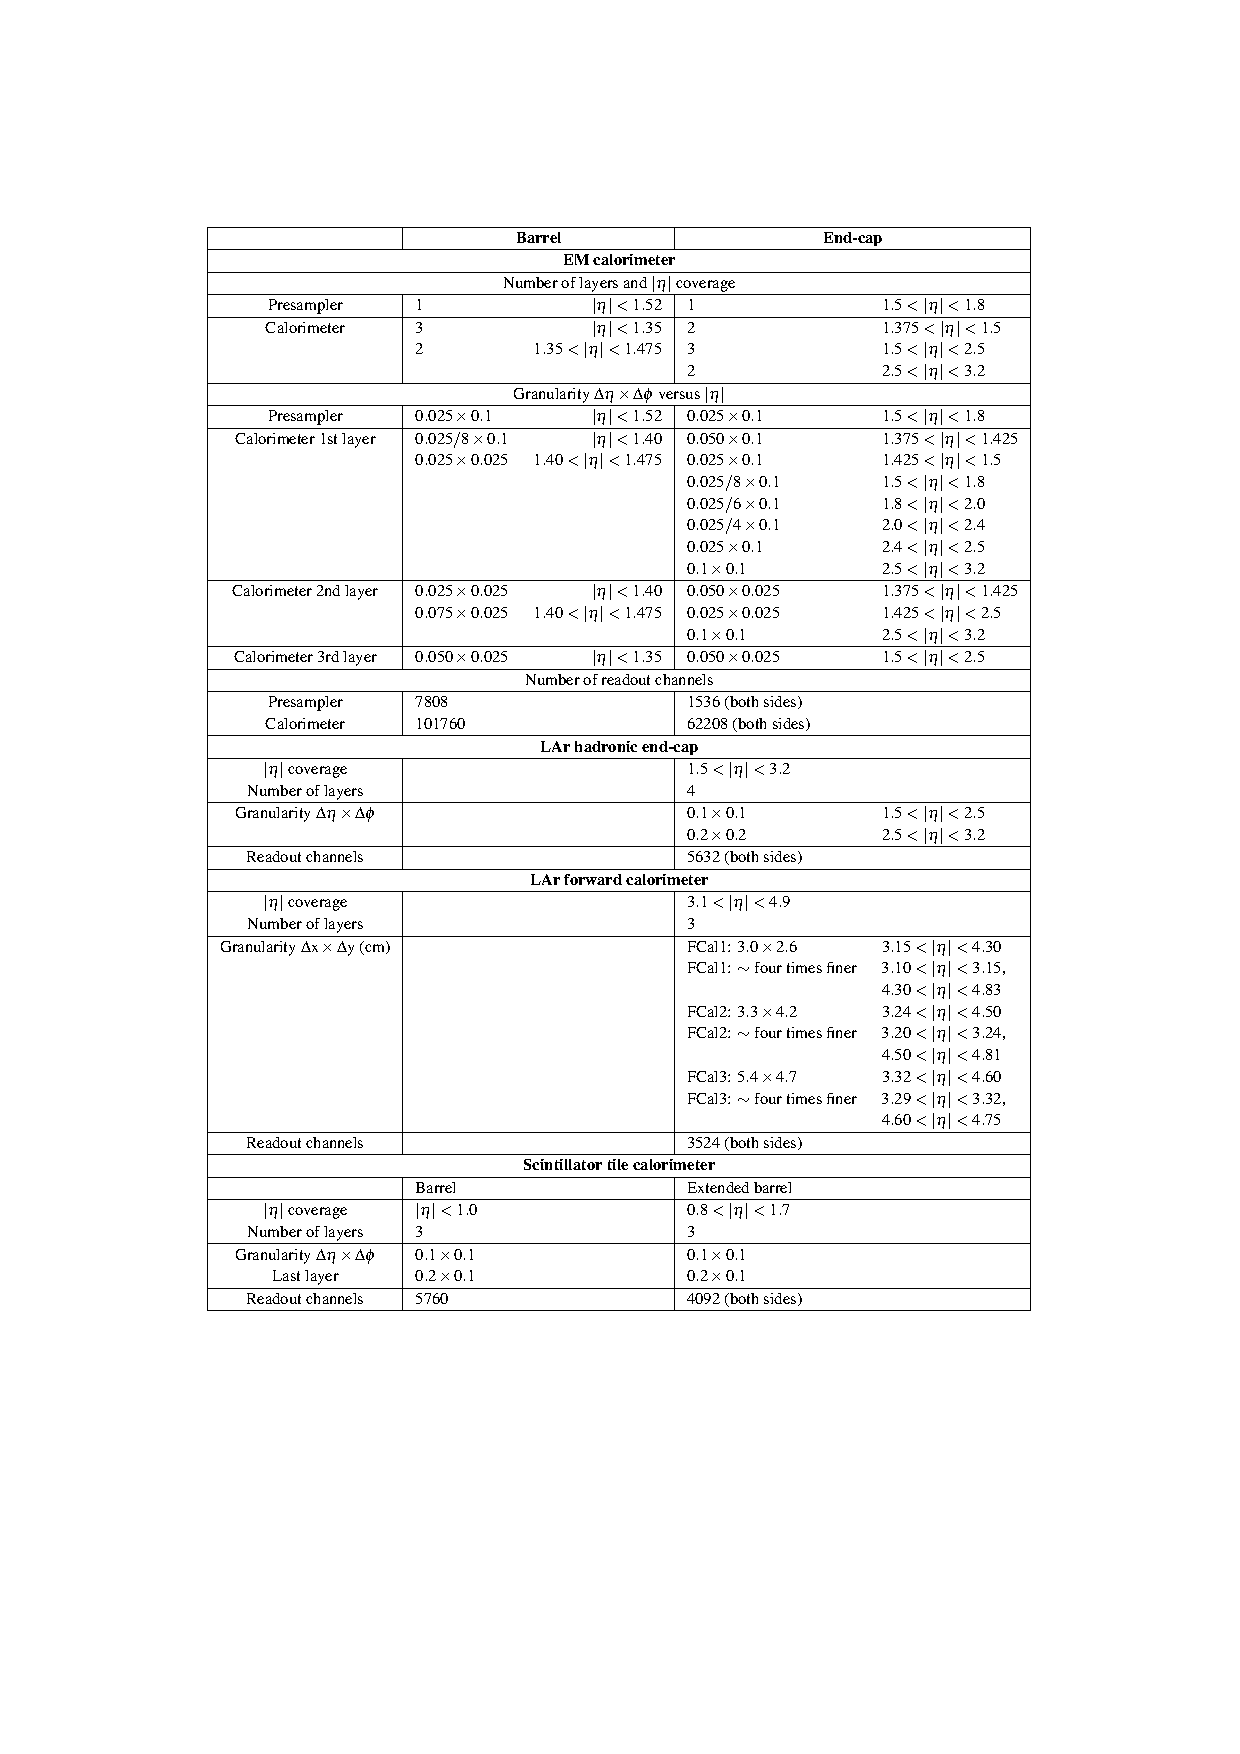
\includegraphics[width=1\linewidth, angle=0]{figs/Detector/tab_calo_granularity.pdf}
%  \end{center}
%  \caption[The key spatial coverage, granularity and readout parameters of the ATLAS calorimeter.]
%          {The key spatial coverage, granularity and readout parameters of the ATLAS calorimeter~\cite{det-ATLAS_Exp}.}
%  \label{tab:det-calo_granularity}
%\end{table}

The ATLAS calorimeter is a non-compensating calorimeter;
which means that the response of the detector to an electromagnetic particle (such as an electron)
is larger than the response to a hadronic particle (for example a pion).
This is because some energy is lost in the hadronic cascade process;
mainly due to the energy required to release nucleons from calorimeter nuclei during spallation \cite{det-comp_calo, det-thesis_lene}.
%but also from the recoil energy given to the calorimeter nuclei
%and neutrinos created during strong processes that can escape the calorimeter \cite{det-comp_calo, det-thesis_lene}.
The ATLAS calorimeter is initially calibrated to the EM-scale,
meaning that the initial energy measurement of a calorimeter assumes that the particle is only EM-interacting.
For hadronic objects a jet energy scale correction is applied,
this is described in Section~\ref{sec:obj-jets_calib}.

\subsubsection{Energy Resolution of a Calorimeter}
\label{sec:det-calo_noise}

The intrinsic energy resolution of a calorimeter is given by three terms:
\begin{equation}
  \left(\frac{\Delta E}{E}\right)^2 = \left(\frac{c_s}{\sqrt{E}}\right)^2 + \left(\frac{c_n}{E}\right)^2 + c_c^2
\end{equation}

\begin{itemize}[leftmargin=*]
\item\textbf{Stochastic Term ($c_s$):}
  This term represents random fluctuations in the cascade shower process.
  $\Delta E_s$ is proportional to the square root of the number of photons/electrons counted in the active layer,
  which means that $\Delta E_s \propto \sqrt{E}$. \vspace{0.5em}
\item\textbf{Noise Term ($c_n$):}
  This term represents uncertainties that are a constant size in units of energy, such that $\Delta E_n = c_n$.
  Contributions to the noise term include electronic noise and effects from pile-up. \vspace{0.5em} % or radioactivity
\item\textbf{Constant Term ($c_c$):}
  This term represents uncertainties that are independent of the energy measurement, such that $\Delta E_c/E = c_c$.
  This uncertainty is mainly caused by the geometry of the calorimeter such as regions of inactive material (detector cracks, material before the calorimeter) and dead modules.
\end{itemize}

Table~\ref{tab:det-calo_noise} shows approximate values of $c_s$ and $c_c$ for the components of the ATLAS calorimeter.
The noise term depends strongly on $\eta$ and pile-up conditions so is not given.
For high-\pT{} objects ($\,\gtrsim 100$ GeV), such as the jets used in di-$b$-jet searches, the constant term is the dominant term,
as the other terms are suppressed by the large values of~$E$.

%{\renewcommand{\arraystretch}{1.2}
%\begin{table}[!htb]
%\centering
%\begin{tabular}{|c||c|c|c|}
%\hline
%Calorimeter Component  & Stochastic ($c_s$) [$\sqrt{\text{GeV}}$]  & Noise  ($c_n$) [GeV]        & Constant ($c_c$)  \\
%\hline
%EM Barrel              & 10\%                                  & $\sim$ 1\%-10\%                  & 0.7\%       \\
%EM End-cap             & 10\%                                  & $\sim$ 1\%-10\%                  & 0.7\%       \\
%Tile                   & 50\%                                  & $\sim$ 10\%-100\%                &   3\%       \\
%HEC                    & 50\%                                  & $\sim$ 10\%-100\%                &   3\%       \\
%FCAL                   & 100\%                                 & $\sim$ 10\%-100\%                &  10\%       \\
%\hline
%\end{tabular}
%\caption[A summary of the stochastic, noise and constant terms of the intrinsic energy resolution of components of the ATLAS calorimeter.]
%        {A summary of the stochastic, noise and constant terms of the intrinsic energy resolution of components of the ATLAS calorimeter.
%        The noise term depends on $\eta$ and pile-up conditions so only an approximate decade is given~\cite{det-ATLAS_Exp,det-thesis_lene}}
%\label{tab:det-calo_noise}
%\end{table}
%}

{\renewcommand{\arraystretch}{1.2}
\begin{table}[!htb]
\centering
\begin{tabular}{|c||c|c|c|}
\hline
\textbf{Calorimeter Component}  & \textbf{Stochastic ($c_s$) [$\sqrt{\text{GeV}}$]}  & \textbf{Constant ($c_c$)}  \\
\hline
EM Barrel              & 10\%                                       & 0.7\%       \\
EM End-cap             & 10\%                                       & 0.7\%       \\
Tile                   & 50\%                                       &   3\%       \\
HEC                    & 50\%                                       &   3\%       \\
FCAL                   & 100\%                                      &  10\%       \\
\hline
\end{tabular}
\caption[A summary of the stochastic and constant terms of the intrinsic energy resolution of components for the ATLAS calorimeter.]
        {A summary of the stochastic and constant terms of the intrinsic energy resolution of components for the ATLAS calorimeter~\cite{det-ATLAS_Exp}}
\label{tab:det-calo_noise}
\end{table}
}

\subsection{Muon Spectrometer}
\label{sec:det-MS}

The Muon Spectrometer (MS) is the outermost part of the ATLAS detector and is designed to measure the trajectory
of charged particles that are not stopped by the calorimeter system.
As the muon is the only charged particle that can pass through the calorimeter system,
measurements in the MS are used to identify muons.
The MS consists of layers of detector providing positional measurements (or hits)
in the presence of a magnetic field, similar to the concept used for the Inner Detector (ID).
%Furthermore, position measurements from both the MS and ID are used to calculate the trajectory of muons,
%known as muon tracks, and from that the momentum of the muon can be inferred.
%By using position measurements from both the MS and the ID, muon tracks have a long lever arm which improves momentum resolution.
Therefore, the trajectory and momentum of muons can be calculated using hits from the MS.
Details of muon reconstruction are discussed further in Section~\ref{sec:obj-leptons}.

In the barrel region ($|\eta|\nobreak<\nobreak1.4$) a large barrel toroid provides the magnetic field,
in the end-cap region ($1.6\nobreak<\nobreak|\eta|\nobreak<\nobreak2.7$) two smaller end-cap magnets  provide the magnetic field
and finally in the transition region ($1.4\nobreak<\nobreak|\eta|\nobreak<\nobreak1.6$) both sets of magnets contribute to the magnetic field.
A further description of the magnets used in ATLAS is found in the next section. 

Muon chambers are the detectors that measure the position of the muon.
In the barrel region,  muon chambers are arranged in three concentric cylindrical layers of chambers formed around the beam-pipe,
whilst in the transition and end-cap regions there are in three disks of chambers perpendicular to the beam-pipe either side of the barrel.

There are two types of muon chambers; trigger and precision.
The trigger muon chambers provide a position measurement in 3-dimensions within 15--\SI{25}{\nano\second} which is used to reconstruct muons in the ATLAS trigger system,
the trigger will be discussed in Chapter~\ref{sec:trig}.
The trigger muon chambers comprise of Resistive Plate Chambers (RPC’s) in the barrel 
and Thin Gap Chambers (TGC’s) in the end-cap regions.
%Only measurements for $|\eta|\nobreak<\nobreak2.0$ are used for triggering due to the high flux of muons close to the beam-pipe.
The precision muon chambers provide a precise measurement of the muon position co-ordinates in the $R$-$z$ plane,
the plane in which trajectory curvature occurs in the MS, allowing for precise measurements of the muon track-$p_T$. 
In the region $|\eta|\nobreak<\nobreak2.0$, the precision muon chambers are entirely Monitored Drift Tubes (MDTs),
whilst at large pseudorapidity ($2.0\nobreak<\nobreak|\eta|\nobreak<\nobreak2.7$) Cathode Strip Chambers (CSCs) are used in addition to MDTs.
A schematic of the MS is shown in Figure~\ref{fig:det-ms_schem}, the types of muon chambers are labelled.

There is an additional use of the MS that relates to high-energy jets.
Whilst for most jets the shower is fully contained within the calorimeter
there are some jets, particularly at high-$p_T$, where a non-negligible amount of energy is not deposited in the calorimeter.
This effect, known as \textit{`punch-through'}, is estimated using energy deposits in the MS.

\begin{figure}[!htb]
  \begin{center}
    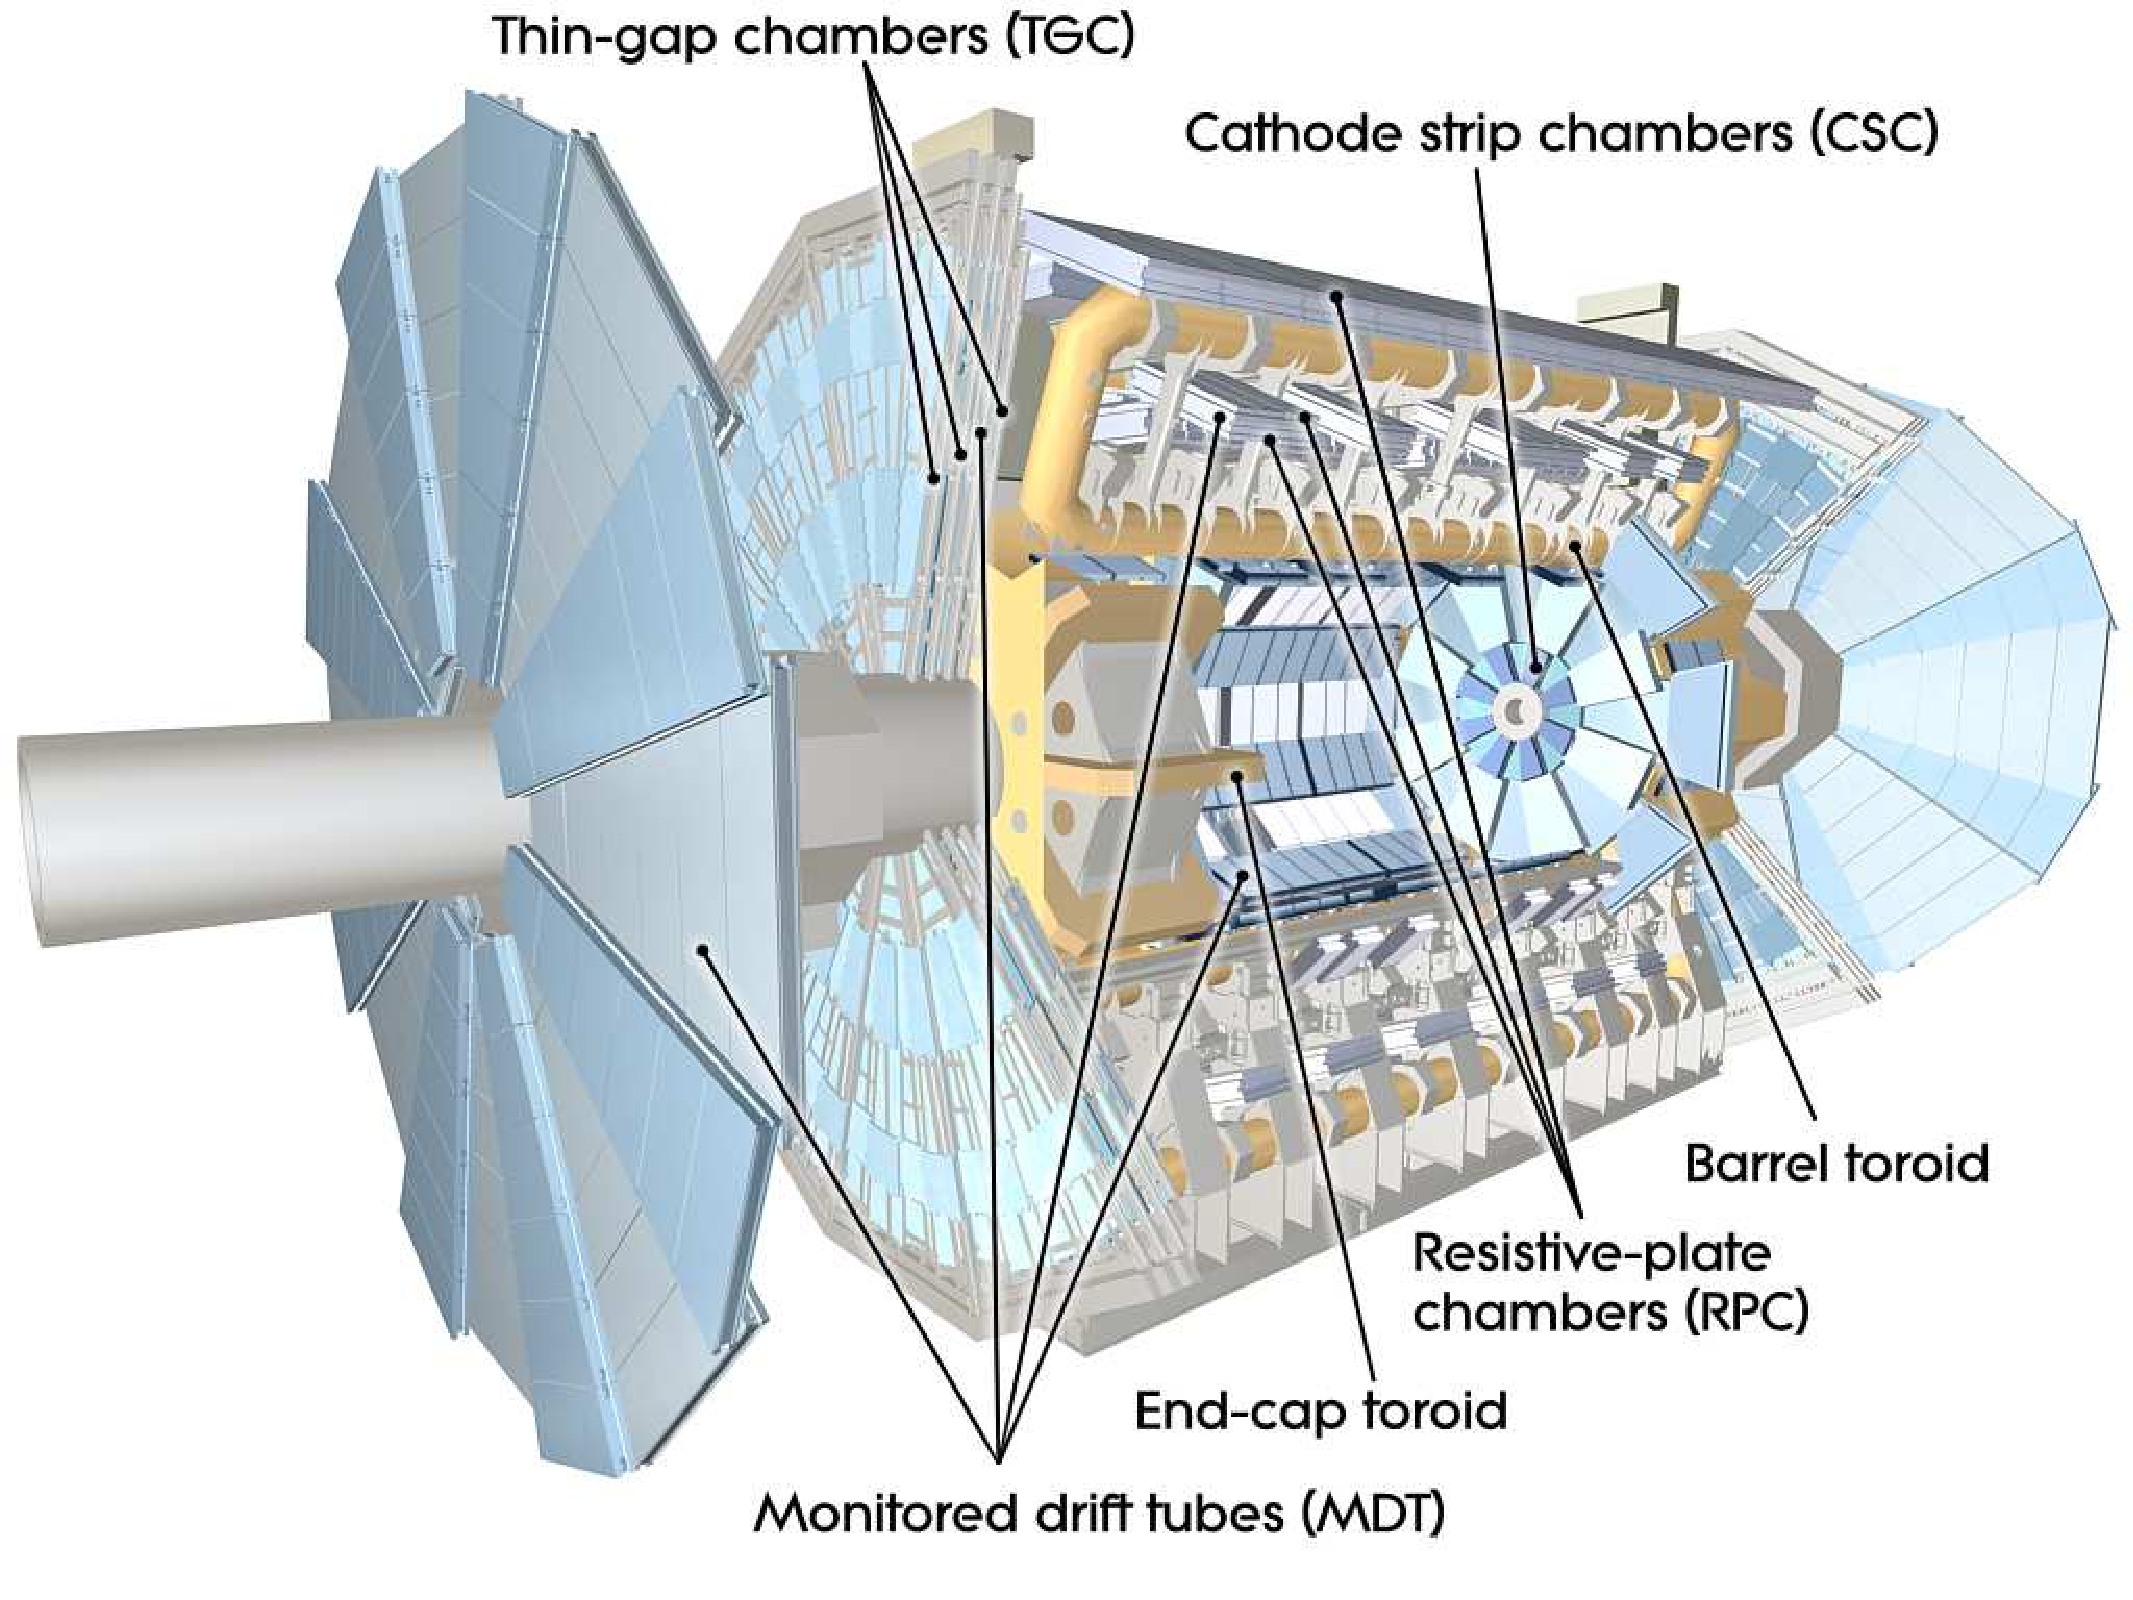
\includegraphics[width=0.8\linewidth, angle=0]{figs/Detector/MS_schem.pdf}
  \end{center}
  \caption[A cut-away of the ATLAS Muon Spectrometer.]
          {A cut-away of the ATLAS Muon Spectrometer (MS). The types of muon chamber used in each part of the MS are labelled on the figure.~\cite{det-ATLAS_Exp}.}
  \label{fig:det-ms_schem}
\end{figure}

\newpage

\subsection{Magnets}
\label{sec:det-magnets}

In ATLAS, magnetic fields are important for obtaining the momentum of particles from their observed trajectories in the ID and MS.
The ATLAS magnet system consists of four large superconducting magnets.
The inner solenoid surrounds the ID and provides a 2~T magnetic field within the ID.
The barrel toroid magnet provides a magnetic field of $\sim$0.5~T in the central regions of the MS and
the two end-cap toroid magnets which produce a magnetic field of $\sim$1~T in the forward regions of the MS.
Figure~\ref{fig:det-magnet_schem} shows the layout of the ATLAS magnet system~\cite{det-magnet_fig}.

\vspace{1em}
\begin{figure}[!ht]
  \begin{center}
    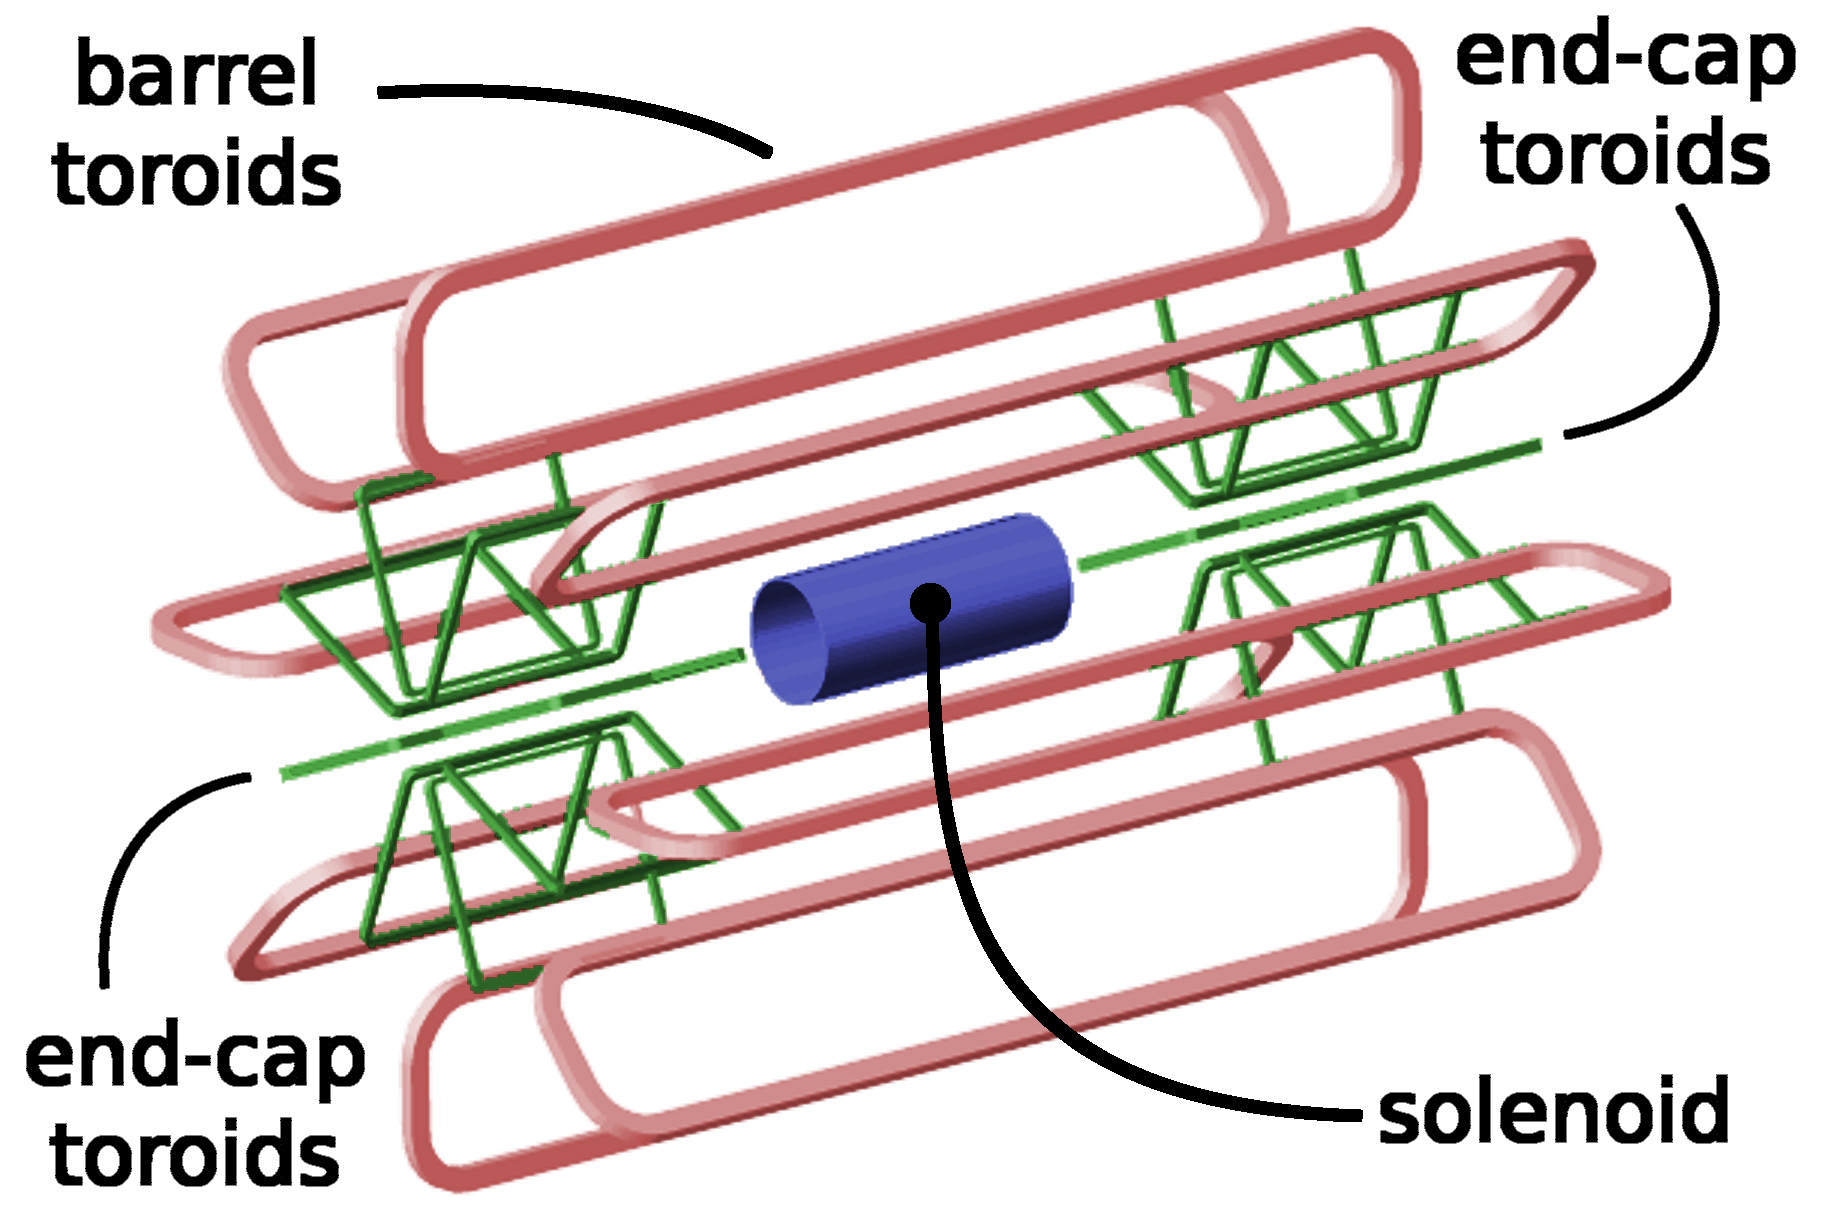
\includegraphics[width=0.8\linewidth, angle=0]{figs/Detector/Magnet_schem.png}
  \end{center}
  \caption[The layout of the ATLAS magnet system.]{The layout of the ATLAS magnet system~\cite{det-magnet_fig}.}
  \label{fig:det-magnet_schem}
\end{figure}

